\documentclass[a4paper,12pt]{article}
\usepackage[english]{babel}
% \usepackage[latin1]{inputenc}
\usepackage[a4paper,margin=0.75in,footskip=0.25in]{geometry}
\usepackage{amsmath}
\usepackage{amssymb}
\usepackage{amsfonts}
\usepackage{graphicx}
\usepackage{listings}
\usepackage[usenames,dvipsnames]{xcolor}
\usepackage{color}
\usepackage{float}
\usepackage[hidelinks]{hyperref}
\usepackage{indentfirst}
\usepackage[utf8]{inputenc}
\newcommand{\link}[1]{{\color{blue}\href{#1}{#1}}}
\usepackage{helvet}
\renewcommand{\familydefault}{\sfdefault}
\usepackage{fancyhdr}
\pagestyle{fancy}
\fancyhf{}
\rhead{Retratista $|$ \textcolor{blue}{2021}}
\rfoot{\thepage $|$ Page}
\renewcommand{\headrulewidth}{0.4pt}
\renewcommand{\footrulewidth}{0.4pt}
\usepackage{arabtex}
\usepackage{utf8}
\usepackage{setspace}
\renewcommand{\baselinestretch}{1.15}
\usepackage{chngcntr}
\counterwithin{figure}{section}
\counterwithin{table}{section}
\usepackage{afterpage}
\usepackage{titlesec}
\setcounter{secnumdepth}{4}
\setcounter{tocdepth}{4}
\titleformat{\paragraph}
{\normalfont\normalsize\bfseries}{\theparagraph}{1em}{}
\titlespacing*{\paragraph}
{0pt}{3.25ex plus 1ex minus .2ex}{1.5ex plus .2ex}

\begin{document}
\setcode{utf8}
\pagecolor{ForestGreen}\afterpage{\nopagecolor}
\begin{titlepage}
%----------------------------------------------------------------------------------------
%	HEADING SECTIONS
%----------------------------------------------------------------------------------------
\newcommand{\HRule}{\rule{\linewidth}{0.5mm}} % Defines a new command for the horizontal lines, change thickness here
\center % Center everything on the page
 
\begin{minipage}{0.45\textwidth}
\begin{flushleft} \large

\includegraphics[scale=0.4]{images/uni-logo.png}\\
\end{flushleft}
\end{minipage}
~
\begin{minipage}{0.45\textwidth}
\begin{flushright}
\end{flushright}
\end{minipage}\\[0.1cm]

\begin{minipage}{0.7\textwidth}
\begin{flushleft}
\hspace*{-2.0cm}
\textsc{Cairo University}\\[0.15cm]
\hspace*{-2.0cm}
\textsc{Faculty of Engineering} \\[0.15cm]
\hspace*{-2.0cm}
\textsc{Department of Computer Engineering} \\
\end{flushleft}
\end{minipage}
~
\begin{minipage}{0.45\textwidth}
\begin{flushright}
\end{flushright}
\end{minipage}\\[1cm]

%----------------------------------------------------------------------------------------
%	TITLE SECTION
%----------------------------------------------------------------------------------------
\begin{minipage}{\textwidth}
\begin{center}
\textbf{\Huge Retratista} \\[0.25cm]
\includegraphics[scale=0.2]{images/logo.png} \\[0.25cm]
A Graduation Project Report Submitted \\[0.1cm]
to \\[0.1cm]
Faculty of Engineering, Cairo University \\[0.1cm]
in Partial Fulfillment of the requirements of the degree \\[0.1cm]
of \\[0.1cm]
Bachelor of Science in Computer Engineering. \\[0.1cm]
\end{center} 
\end{minipage} \\[1cm]
 
%----------------------------------------------------------------------------------------
%	AUTHOR SECTION
%----------------------------------------------------------------------------------------
\begin{minipage}{\textwidth}
\begin{center}
\textbf{\Large Presented by}
\end{center} 
\end{minipage} \\[0.5cm]

\begin{minipage}{0.45\textwidth}
\begin{center} 
Mohamed Shawky Zaky AbdelAal Sabae \\[0.5cm]
Mohamed Ahmed Mohamed Ahmed
\end{center}
\end{minipage}
~
\begin{minipage}{0.45\textwidth}
\begin{center}
Remonda Talaat Eskarous \\[0.5cm]
Mohamed Ramzy Helmy Ibrahim
\end{center}
\end{minipage} \\[1cm]

\begin{minipage}{\textwidth}
\begin{center}
\textbf{\Large Supervised by}
\end{center} 
\end{minipage} \\[0.5cm]

\begin{minipage}{0.45\textwidth}
\begin{center} 
Dr. Mayada Hadhoud
\end{center}
\end{minipage} \\[1cm]

\begin{minipage}{0.45\textwidth}
\begin{center} 
26th July, 2021
\end{center}
\end{minipage} \\[0.5cm]

\begin{minipage}{\textwidth}
\begin{center} 
\small All rights reserved. This report may not be reproduced in whole or in part, by photocopying or other means, without the permission of the authors/department.
\end{center}
\end{minipage}

\end{titlepage}

%----------------------------------------------------------------------------------------
%	REPORT SECTIONS
%----------------------------------------------------------------------------------------

\section*{Abstract}
Throughout history, \emph{portraiture} has been a mean of identifying and finding individuals due to various reasons. Aside from being an art to memorialize famous historical characters, it has been used to identify criminals and missing individuals. The main reason behind using portraits for these purposes is that \emph{visual search} is much easier for humans than any other kind of search. Most people can identify a person or an object, they have seen before. Even with the rise of photography, statistics say that drawn portraits are still used in visual search. Recently, portraits developed other applications as well, especially in the study of historical characters and events.

While being important, sketching a complete face portrait can be very cumbersome and time-consuming. Historically, this process required a professional portraitist and could take him weeks to fully sketch an accurate portrait. However, with the rise of digital design application including \emph{Adobe Photoshop}, this process became much easier. Nonetheless, it still requires a professional and can take hours or even days to accomplish. Moreover, the process of refining a drawn portrait can be very tedious and can cause re-sketching in certain cases. On the other hand, the process of sketching a portrait sometimes needs to be extremely fast, in cases of searching for dangerous criminals or missing children. 

\textbf{Retratista} addresses both \emph{time} and \emph{accuracy} issues, while keeping the usage as simple as possible for non-professionals. We use the power of modern \emph{generative models} to create an \emph{end-to-end} system for \emph{face portrait generation} from bare description. This description can be a voice, text or manual description. We abstract the complexity of our system from the user by providing a simple \emph{web user interface}. Our system takes just a \emph{few seconds} to generate a complete face. Also, it allows the user to further \emph{refine} the generated face and even render it in \emph{multiple poses} to provide further identification. We include a relatively-sufficient set of \emph{facial attributes} to correctly describe a human face.

\addcontentsline{toc}{section}{Abstract (English)}

\newpage

\begin{arabtext}
{\LARGE
الملخص
}\vspace{20pt}
على مر التاريخ ،كان فن البورتريه وسيلة للتعرف والعثور على الأفراد لأسباب مختلفة. بصرف النظر عن كونه فنًا لإحياء ذكرى الشخصيات التاريخية الشهيرة، فقد تم استخدامه لتحديد المجرمين والأفراد المفقودين. السبب الرئيسي وراء استخدام الصور الشخصية لهذه الأغراض هو أن البحث المرئي أسهل بكثير على البشر من أي نوع آخر من البحث. يمكن لمعظم الناس التعرف على شخص أو شيء ما، رأوه من قبل. حتى مع ظهور التصوير الفوتوغرافي، تشير الإحصائيات إلى أن الصور المرسومة لا تزال تستخدم في البحث المرئي. في الآونة الأخيرة، طورت البورتريهات تطبيقات أخرى أيضًا، لا سيما في دراسة الشخصيات والأحداث التاريخية.

على الرغم من أهميته، إلا أن رسم صورة كاملة للوجه يمكن أن يكون مرهقًا جدًا ويستغرق وقتًا طويلاً. تاريخياً، تطلبت هذه العملية رسام بورتريه محترف ويمكن أن تستغرق أسابيع لرسم صورة دقيقة بالكامل. حاليا ومع ظهور تطبيقات التصميم الرقمي مثل Adobe Photoshop، أصبحت هذه العملية أسهل بكثير. ومع ذلك، لا يزال الأمر يتطلب متخصصًا ويمكن أن يستغرق ساعات أو حتى أيامًا لإنجازه. علاوة على ذلك، قد تكون عملية تحسين الصورة المرسومة صعبة للغاية ويمكن أن تؤدي إلى إعادة الرسم في حالات معينة. من ناحية أخرى، يجب أن تكون عملية رسم البورتريه سريعة للغاية في بعض الأحيان، في حالات البحث عن مجرمين خطرين أو أطفال مفقودين.

يعالج ريتراتيستا مشكلات الوقت والدقة، مع الحفاظ على سهولة الاستخدام قدر الإمكان لغير المتخصصين. نحن نستخدم قوة النماذج التوليدية الحديثة لإنشاء نظام شامل لتوليد صورة الوجه من الوصف العاري. يمكن أن يكون هذا الوصف صوتًا أو نصًا أو وصفًا يدويًا. نحن نعزل تعقيد نظامنا عن المستخدم من خلال توفير واجهة مستخدم ويب بسيطة. يستغرق نظامنا بضع ثوانٍ فقط لتكوين وجه كامل. كما أنه يسمح للمستخدم بتحسين الوجه الذي تم إنشاؤه بشكل أكبر وحتى عرضه في أوضاع متعددة لتوفير مزيد من التعريف. نقوم بتضمين مجموعة كافية نسبيًا من سمات الوجه لوصف الوجه البشري بشكل صحيح.

\end{arabtext}
\addcontentsline{toc}{section}{Abstract (Arabic)}

\newpage

\section*{Acknowledgement}
First of all, we would like to express our deep gratitude to our supervisor \textbf{Dr. Mayada Hadhoud} for providing us with incredible guidance and support and making this work possible. Also, we like to thank \textbf{Prof. Albert Gatt} and \textbf{Dr. Marc Tanti} from \emph{University of Malta} for providing us with necessary dataset used in initial experimentation. Also, we would like to thank all the professors, lecturers and teaching assistants in our department for guidance and support throughout the college year. Last but not least, we would like to thank our families for always providing awesome support.
\addcontentsline{toc}{section}{Acknowledgement}

\newpage

\tableofcontents
\addcontentsline{toc}{section}{Table of Contents}

\newpage

\listoffigures
\addcontentsline{toc}{section}{List of Figures}

\newpage

\listoftables
\addcontentsline{toc}{section}{List of Tables}

\newpage

\section*{List of Abbreviation}
\begin{tabular}{l l}
AI & Artificial Intelligence \\
ML & Machine Learning \\
DL & Deep Learning \\
NLP & Natural Language Processing \\
CNN & Convolutional Neural Network \\
RNN & Recurrent Neural Network \\
GAN & Generative Adversarial Network \\
API & Application Programming Interface \\
FFHQ & Flickr-Faces-HQ Dataset \\
ADA & Adaptive Discriminator Augmentation \\
FID & Fréchet Inception Distance \\
LPIPS & Learned Perceptual Image Patch Similarity \\
AdaIN & Adaptive Instance Normalization \\
GPU & Graphics Processing Unit \\
TPU & Tensor processing unit
\end{tabular}
\addcontentsline{toc}{section}{List of Abbreviation}

\newpage

\section*{List of Symbols}
\begin{tabular}{l l}
$||A||$ & Magnitude of a Vector $A$ \\
$Trace(B)$ & Trace of a Matrix $B$ \\
$D$ & Feature Directions Matrix \\
$d$ & Single Feature Direction Vector \\
$E$ & Face Embedding (Latent Vector) \\
$l$ & Logit (Numerical Value) \\
$l_{diff}$ & Differentiated Logits (Result of Logits Subtraction)
\end{tabular}
\addcontentsline{toc}{section}{List of Symbols}

\newpage

\section*{Contacts}
\textbf{\large Team Members}

\begin{tabular}[t]{|l |l |l |}
\hline
Name & Email & Phone Number \\
\hline \hline
Mohamed Shawky Zaky & \link{mohamedshawky911@gmail.com} & +2 01271194141 \\
\hline
Remonda Talaat Eskarous & \link{remondatalaat21@gmail.com} & +2 01554753224 \\
\hline
Mohamed Ahmed Mohamed & \link{mohammed.ahmed.m.228@gmail.com} & +2 01090666536 \\
\hline
Mohamed Ramzy Helmy & \link{mohamedramzy98620@gmail.com} & +2 01153302514 \\
\hline
\end{tabular} \\[1cm]

\textbf{\large Supervisor}

\begin{tabular}[t]{|l |l |l |}
\hline
Name & Email & Phone Number \\
\hline \hline
Dr. Mayada Hadhoud & \link{mayadahadhoud@gmail.com} & +2 01099957167 \\
\hline
\end{tabular}

\addcontentsline{toc}{section}{Contacts}

\newpage

\

\newpage

\section{Introduction}
Face portrait has been used for multiple important tasks related to visual search and study. Visual search of criminals and missing individuals is completely based on visual face portraits. Having an accurate face portrait can enable automated and efficient search through camera feeds and even faster manual search. Also, face portraits are the bases of the many studies related to history and archaeology. Despite of its importance, the process of generating a portrait from bare description is tedious and time-consuming. Traditionally, this process is done by professional portraitists that manually sketch the face portrait. This can take days or weeks to accomplish using traditional sketching and hours using digital sketching. In some cases, this can be unacceptable.

\texttt{Retratista} addresses the problem of \emph{face portrait generation} from \emph{various descriptions}. These descriptions include voice, textual and manual descriptions. We design our system for complete \emph{automated} portrait generation, with a simple \emph{web user interface}. Moreover, rapid face refinement and rotation is provided to further improve face identification. Our system solves both duration and complexity issues of previous portrait sketching methods, while providing a high fidelity results and keeping simple interface. This eases the usage of portraits in many applications.

\texttt{Retratista} combines the power of modern \emph{AI} solutions and the great applications of portraiture into a single tool that is available for everyone to use efficiently without experience and with minimum duration. 

\subsection{Motivation and Justification}
Sketching a human face from bare description is a tedious task that requires specialization. Normally, professional portraitists are asked to sketch a face from description. The process of sketching a human face portrait from scratch can involve problems, such as :
\begin{itemize}
    \item A long time to initially sketch the face that matches the description.
    \item After being sketched, any refinements in the face might require re-sketching from scratch.
    \item Sketched faces are not accurate and real enough to be used for facial recognition in both manual and automated (\emph{AI-driven}) visual search.
\end{itemize}

Despite its difficulty, the process of sketching portrait has many applications, most of which require high accuracy and speed. These applications include :
\begin{itemize}
    \item Visual search of missing individuals and criminals.
    \item Visualization of historical and mythical characters.
    \item Search of surveillance video feeds for individuals' actions.
\end{itemize}

Here are some statistics from \emph{International Centre For Missing and Exploited Children} (ref: \link{https://www.icmec.org}) that can tell how our system is critically needed :

\begin{itemize}
    \item In \textbf{USA}, an estimated \textbf{460,000} children are reported missing every year.
    \item In \textbf{UK}, an estimated \textbf{112,853} children are reported missing every year.
    \item In \textbf{Germany}, an estimated \textbf{100,000} children are reported missing each year.
    \item In \textbf{India}, an estimated \textbf{96,000} children go missing each year.
    \item In \textbf{Canada}, an estimated \textbf{45,288} children are reported missing each year.
    \item In \textbf{Russia}, an estimated \textbf{45,000} children were reported missing in 2015.
    \item In \textbf{Australia}, an estimated \textbf{20,000} children are reported missing every year.
    \item In \textbf{Spain}, an estimated \textbf{20,000} children are reported missing every year.
\end{itemize}

All cases of missing individuals require a visual face image to ease the search process. Most of them require sketching a face portrait (either for the missing person or a potential suspect), even with all the advances in photography.

\subsection{Project Objectives and Problem Definition}
The main focus of \textbf{Retratista} is to offer as many utilities as possible to identify a human face from any description. To do this, we have to :
\begin{itemize}
    \item Translate the input description to a complete human face image.
    \item Refine the generated face image, as needed, in order to reach the target face.
    \item Render the final face in multiple poses to provide more face identification.
\end{itemize}

In order for our product to be valuable, these functionalities have to be done as fast as possible, while maintaining output accuracy and quality. Also, it should be an \emph{easy-to-use} interface with no required experience to use, only enter the description and edit what is needed. The output of our system can, then, be used in multiple applications of visual search and identification.

\subsection{Project Outcomes}
The project outcome is a web application that simply takes a description as voice, text or manual input and translates it into a complete realistic face portrait within a \emph{few seconds} in a \emph{fully-automated} way. Then, the application gives the user a chance to further refine the facial attributes to match the target face. Furthermore, the generated face can be rendered in multiple poses for better identification. Our system considers $32$ facial attributes for generation and $38$ facial attributes for refinement. The facial attributes include \emph{age}, \emph{gender}, \emph{hair color} and \emph{eyes color}. 

\subsection{Document Organization}
The document is organized into $6$ chapters along with the appendices. Chapter $1$ introduces the main idea of the project, along with the formal definition of the problem, our motivation to work on this problem and the project outcome.

Chapter $2$ discusses the market study of our project through identifying the target market and listing our potential competitors. Also, it provides a financial analysis for our product.

Chapter $3$ gives the necessary background information, along with previous related work in research literature and shows our adopted approach.

Chapter $4$ is the main body of our document, where it discusses, in details, our system architecture and application design. This chapter further explains the implementation details of our modules. Finally, it discusses alternative approaches considered in our experimentation.

Chapter $4$ explains the metrics, used to assess our system, and our system results. The testing is described both qualitatively and quantitatively. Also, we show the success and failures cases of our system.

Chapter $5$ concludes our document, lists the faced challenges and shows how our work can be extended and improved.

Finally, we include $4$ appendices for describing development tools, project use cases, user guide and product feasibility study.


\newpage

\section{Market Feasibility Study}

Face Generation is an important field in the market, it is used widely in all camera applications to apply filters on the taken images most of the usage was for entertainment, Although it can be used to have photos for any missing people or criminal and that will increase the chance to find that missing people or the criminal.
 
\subsection{Targeted Customers}
Our Project is directed to all governmental and volunteering organizations, that need to generate identical faces of missing people from bare human description of their facial features.
It also can be used to identify the ancient kings and queens faces from the Papyrus .
We can categorize the different target companies into the following:
\begin{itemize}
    \item \textbf{Criminal identification from witnesses descriptions :}
        \begin{itemize}
            \item INTERPOL.
            \item Different Police Stations.
        \end{itemize}
    \item \textbf{Missing People organizations like :}
        \begin{itemize}
            \item International Center for Missing and Exploited Children.
            \item International Red Cross and Red Crescent Movement.
            \item International Commission on Missing Persons \emph{ICMP}
            \item The Doe Network.
            \item National Missing and Unidentified Persons System.
            \item Missing Persons Support Center.
            \item Be United Missing Persons Inc.
            \item others.
        \end{itemize}
    \item \textbf{Historical Characters Identification :}
        \begin{itemize}
            \item Archaeological and Historical Research Facilities.
        \end{itemize}
\end{itemize}

\subsection{Market Survey}

As mentioned previously, most Applications that uses face generation is for entertainment, So they depends only on image refinement on limited number of features to generate the image unlike us, We have both image generation and refinement using 34 features for generation and 38 for refinement.
Besides that our goal is to find missing person for purpose more important than entertaining. Our biggest competitor is FaceApp, followed by PicsArt, Facetune2 and Booth Apps.
  

\subsubsection{FaceAPP}

\begin{figure}[H]
    \centering
    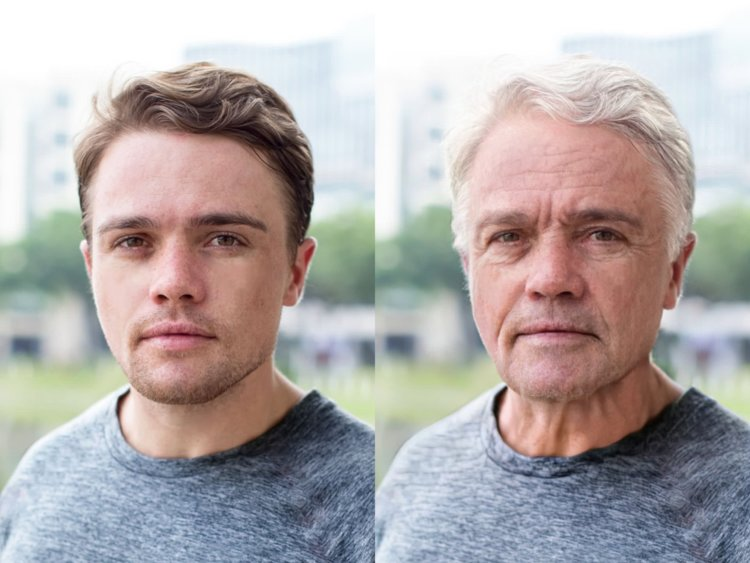
\includegraphics[width=0.6\textwidth]{images/FaceApp.jpg}
    \caption{Changing Age using FaceApp application.}
    \label{fig:faceApp}
\end{figure}

\emph{FaceAPP} is considered Image and video editing mobile application, it generates highly realistic transformations of human faces in photographs using AI and Neural Networks. 
The Limitation of the App compared with us, it only used for refinement using 14 facial feature which may be not enough for generating face from scratch.

\subsubsection{PicsArt}

\begin{figure}[H]
    \centering
    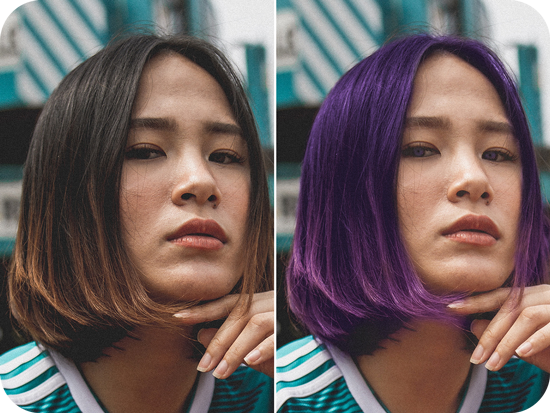
\includegraphics[width=0.6\textwidth]{images/picsArt.png}
    \caption{image refinement using PicsArt application.}
    \label{fig:picsArt}
\end{figure}

\emph{PicsArt} is a company that develops online photo and video editing applications, with a social creative community. The platform allows users to take and edit pictures and videos and draw with layers. It only allows 9 features refinement so it's also not the best choice for image generation.

\subsubsection{Facetune2}

\begin{figure}[H]
    \centering
    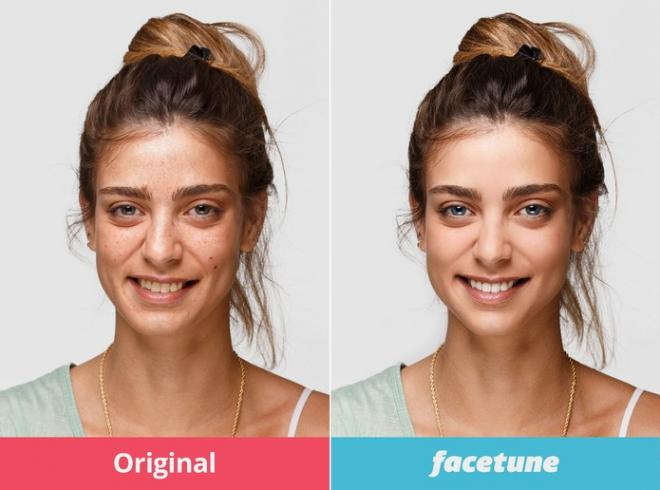
\includegraphics[width=0.5\textwidth]{images/FaceTune.jpg}
    \caption{image refinement using FaceTune2 application.}
    \label{fig:FaceTune2}
\end{figure}

\emph{Facetune2} is a photo editing application. It's commonly used to enhance the portrait o selfie images and offers 7 feature refinements.

\subsubsection{Booth Apps}

\begin{figure}[H]
    \centering
    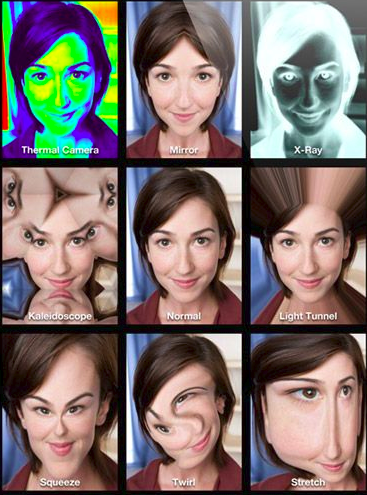
\includegraphics[width=0.5\textwidth]{images/photoBooth.png}
    \caption{image Editing using PhotoBooth application.}
    \label{fig:photoBooth}
\end{figure}

\emph{Booth Apps} are a collection of applications for image or video editing and enhancement, can add animation to an image and many other entertaining features. Examples for Booth Apps are : Simple Booth Classic, Mini Photobooth, Pocketbooth, Photobooth mini and My Photobooth App.
They only consider image enhancement and for entertaining purposes not critical issues like our product.

\subsection{Business Case and Financial Analysis }

Our product is new in the market which makes our business case a good one. We can provide our services in two forms as following:
\begin{itemize}
    \item The first is being a software service that is used in police stations so that any missing people or theft happens, they enters the description of that person so they can have an image for him/her to be able to find him faster, Or used in historical institutions that is responsible for finding information about the history from papyrus.
    \item The second one is a website for general users to be able to use it to generate images for their ancestors who died without having any images, from their parents' descriptions so they can see them, or for any entertaining purposes.
\end{itemize}

The financial analysis of this application is done after detailed market research.
The cost estimation for our software as a service in a specific institution is the cost behind the hardware, our application takes around 1 second on an \emph{Nvidia GTX 1080 ti} for generating the face from any description, but this can extend to be multiple seconds based on the connection. The whole system can be deployed on single PC with 11GB VRAM, around 700\$ for the GPU and 1500\$ to 2000\$ for the whole PC. For scalability, we can use 2 PCs one for generation and the other for Pose estimation to host the whole application. Also, we can scale out our system on more than 2 PCs for improved request parallelism. For the second type of usage we can deploy the system on cloud instance which costs around 150\$ per month for these specifications.


\newpage

\section{Literature Survey}
In this chapter, we explain the necessary background, as well as the related work in the research literature.

\subsection{Background Review}
We discuss the basic background knowledge that helps us throughout the document.

\subsubsection{Convolutional Neural Networks}
First we do a brief introduction for Convolutional Neural Networks (CNN). CNN is a special type of \emph{feed-forward} neural networks, which uses convolution operations to perform the forward computations. They are used in wide range of applications, especially \emph{computer vision}. There are $4$ basic types of layers in a CNN that we would like to mention :
\begin{enumerate}
    \item \textbf{Convolution layer} : uses filters (a.k.a. \emph{kernels}) to detect edges and shapes by convolution with the input map. The filter has certain dimensions and scans the map using certain stride. This helps the network to learn sparse connections and local structures.
    \item \textbf{Pooling layer} : is usually used to reduce the input dimensions through maximizing or averaging using a filter.
    \item \textbf{Upsampling layer} : increases the dimensions of the input map using traditional upsampling methods, such as bilinear upsampling, or learnable upsampling using \emph{deconvolution}.
    \item \textbf{Fully-connected layer} : is a normal feed-forward dense layer, usually used in classification.
\end{enumerate}

\subsubsection{Generative Adversarial Networks}
Generative Adversarial Networks (\emph{GANs}) \cite{goodfellow2014generative} are generative models that can learn through \emph{adversarial training}. GANs have proven to be very good at generating high dimensional data like images. That's why they are used in wide range of applications including image and video generation, image-to-image translation and others.

\begin{figure}[H]
    \centering
    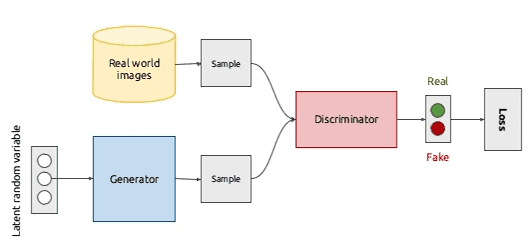
\includegraphics[width=0.8\textwidth]{images/gan-arch.png}
    \caption{The basic architecture of a generative adversarial network (GAN).}
    \label{fig:gan}
\end{figure}

The basic architecture of a GAN (as shown in \ref{fig:gan}) consists of $2$ main networks. A \emph{generator} takes in random noise (usually \emph{latent random variable}) and convert it into a fake data sample. A \emph{discriminator} judges the quality of the fake data sample by distinguishing between real and fake data samples. The discriminator loss (a.k.a. \emph{adversarial loss}) is used to train both generator and discriminator. So, the whole system can be decomposed into a two-player \emph{minimax} formulated as :
\begin{equation}
    min_{G} max_{D} V(D, G) = E_{x \sim Pdata}(x) [log D(x)] + E_{z \sim Pz}(z)[log(1 - D(G(z)))]
\end{equation}

The generator and discriminator networks can be any type of networks. In our case, we use \emph{Convolutional Neural Networks} (CNN), because the output is an image. Consequently, the generator is a CNN that up-samples the latent variable into a complete image. Meanwhile, the discriminator is a classification CNN that encodes the input image and classifies it into real or fake.

The first architecture for a CNN-based GAN goes by the name \texttt{DCGAN} \cite{radford2016unsupervised}. In our work, we focus on a specific type of GANs, named \emph{style-based} (or \emph{latent-based}) GANs.

\subsubsection{Latent Space and Entanglement}
As mentioned before, we focus on a specific type of generative models named \emph{style-based} GANs. These GANs can have artistic control over their outputs, not just sampling data randomly from a prior distribution. The key idea of these models is to use a \emph{latent variable} to control the output, instead of just considering a random noise. This latent variable is sampled from a \emph{latent space} and, then, used to guide the generation process in the generator network using adaptive instance normalization (\emph{AdaIN}).

\emph{AdaIN} is a normalization method that aligns the mean and variance of the content features with those of the style features. It's an extension over \emph{Instance Normalization}, which normalizes the input to a single style specified by the affine parameters. It can be formulated as follows :
\begin{equation}
    AdaIN(x,y) = \sigma(y)(\frac{x - \mu(x)}{\sigma(x)}) + \mu(y)
\end{equation}

The latent space is a made-up space, in which the data is encoded in low dimensional representation. For a good model architecture, the latent space is organized, such that similar features are clustered together and changes in low dimensional latent space maps to similar changes in the generated data. Some the most popular and robust latent-based architectures are \texttt{BigGAN} \cite{brock2019large} and \texttt{StyleGAN} \cite{karras2019stylebased} \cite{karras2020analyzing}. 

\begin{figure}[H]
    \centering
    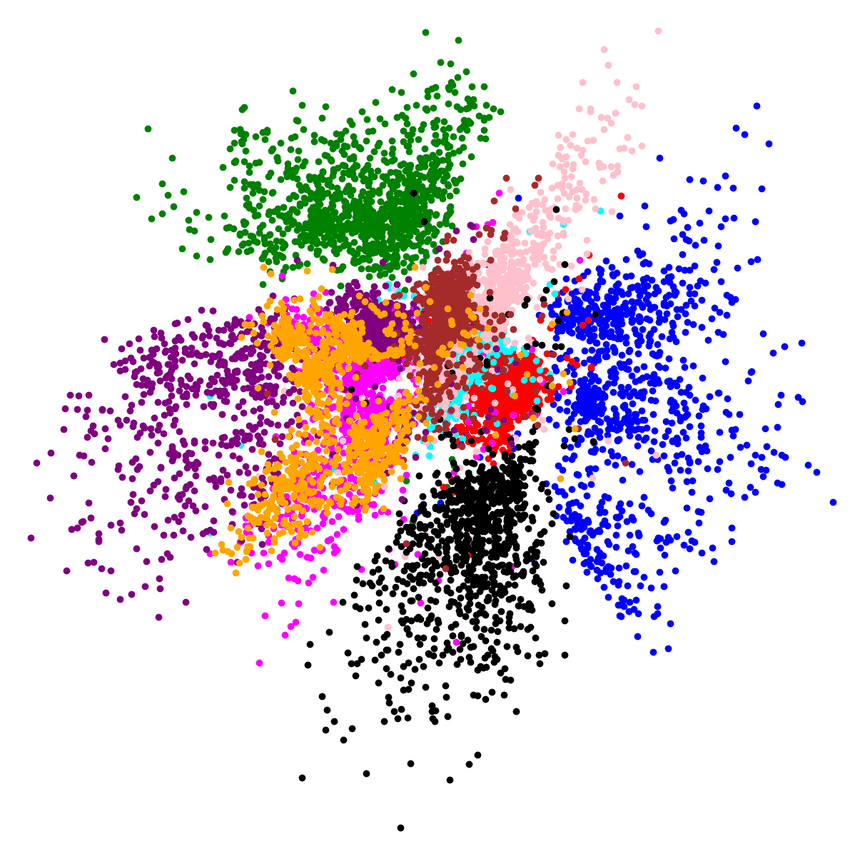
\includegraphics[width=0.6\textwidth]{images/latent-space.png}
    \caption{An example 2D latent space of MNIST digits dataset.}
    \label{fig:lspace}
\end{figure}

Figure \ref{fig:lspace} shows a simple $2D$ latent space for \texttt{MNIST} dataset for digits classification. We can see that we have $10$ clusters corresponding to the $10$ digits. Some clusters are more overlapping than others. It's obvious from the figure that we can learn certain directions to move from one cluster to another in the latent space. However, due to overlapping, certain directions might not be clear or even feasible to obtain. This problem is known as \textbf{entanglement}, which is one of the most important challenges of our work.

The problem of entanglement arises due to the data and training process of the architecture. Some datasets can show heavy correlation between different features, which causes the latent space to be less organized and the features clusters to be overlapping. Thus, the features are entangled in the latent space and extracting independent directions for every feature is hard or even infeasible. Consequently, moving along a certain direction can cause multiple features to change with certain amounts.

\subsubsection{Multi-class Multi-label Text Classification}

\subsection{Face Modelling and Generation}
In this sub-section, an overview is given about face generation and refinement methods.

\subsubsection{Face Generation}
The problem of human face generation is not new to the \emph{AI} research. Many generative models target the problem of face generation from scratch.

\paragraph{StyleGAN}
A new generator architecture is proposed that enables controlling the synthesis of the faces by learning the unsupervised separation of high level features. It generates a complete high quality face image controlled by the latent code. It basically works as follows :
\begin{itemize}
    \item Latent code first is mapped to an intermediate latent space.
    \item The intermediate latent code controls the generator using adaptive instance normalization.
\end{itemize}

\paragraph{Visual Results}
\begin{figure}[H]
    \centering
    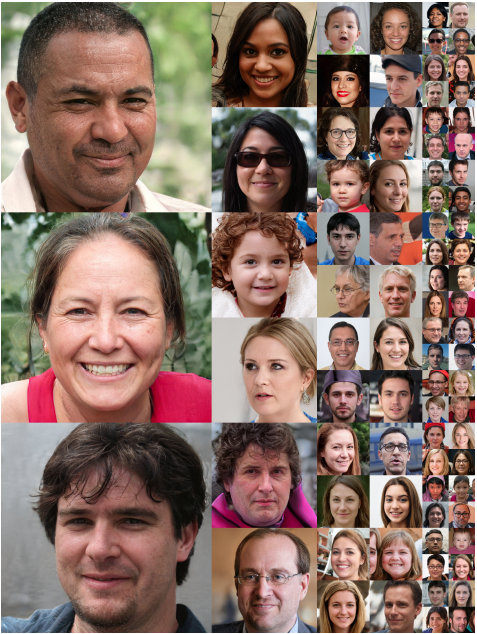
\includegraphics[width=0.6\textwidth]{images/stylegan-results.png}
    \caption{Visual results of StyleGAN2.}
    \label{fig:stgan_res}
\end{figure}

Figure \ref{fig:stgan_res} shows visual result samples from \texttt{StyleGAN2}, which is the revisited version of \texttt{StyleGAN}.

\paragraph{StyleGAN latent manipulation}
Subsequent research work follows \texttt{StyleGAN} to try latent manipulation for more control over the generated faces. These methods include \texttt{Image2StyleGAN} \cite{abdal2019image2stylegan}, \texttt{Image2StyleGAN++} \cite{abdal2020image2stylegan}, \texttt{InterfaceGAN} \cite{shen2020interfacegan}, \texttt{StyleRig} \cite{tewari2020stylerig} and \texttt{StyleFlow} \cite{abdal2020styleflow}. All of these work targeted the directed manipulation of \emph{StyleGAN} latent space to change certain facial features. However, none of these methods target complete generation of new face from bare description, which is, also, known as \emph{conditioned sampling}. 

On the other hand, our work target face generation from bare description. Consequently, we utilize the concept of directed manipulation to do conditioned sampling, which is described later in this document.

\paragraph{Faces à la Carte}
To our knowledge, this \cite{wang2020faces} is the only current open-source research work that addressed the problem of face generation from text. It's based on \texttt{StyleGAN2} and uses a general framework to extract the feature directions and reach the target face.

We couldn't replicate their results, because the authors don't provide sufficient information about their method. However, we managed to gain some insights that helped us throughout the project.

\begin{figure}[H]
    \centering
    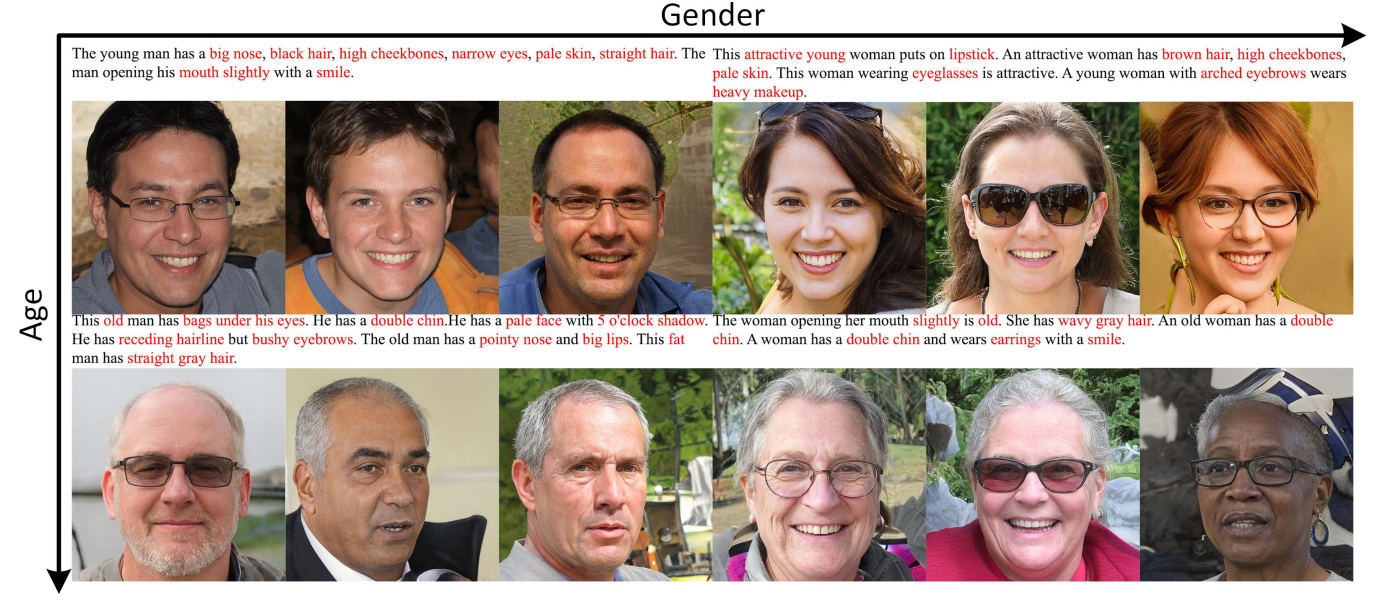
\includegraphics[width=\textwidth]{images/face-carte.png}
    \caption{Visual results of Faces à la Carte.}
    \label{fig:face_carte}
\end{figure}

Figure \ref{fig:face_carte} shows the visual results that the authors included in their paper. While being conservative about some of their work, we still consider this as the only former open-source research work related to our problem.

\paragraph{NVAE}
The paper \textbf{NVAE: A Deep Hierarchical Variational Autoencoder} \cite{vahdat2021nvae} is a recent research work that discusses the usage of Variational Autoencoder (\emph{VAE}) to generate high quality image controlled by a latent variable. It uses normalizing flows to control the output features. \emph{Normalizing flows} is a method of mapping an unknown distribution to a known distribution (normal or uniform). It's basically used to generate complex distributions from simple normal distributions.

\begin{figure}[H]
    \centering
    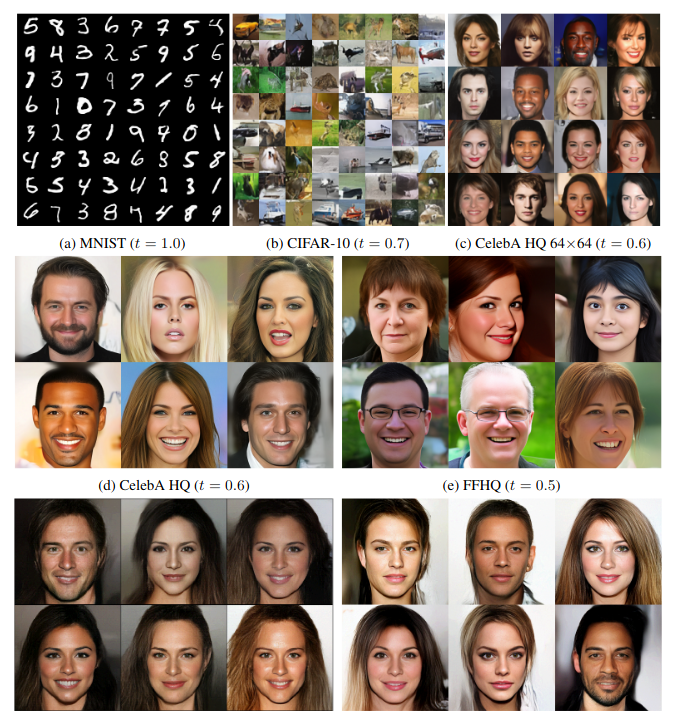
\includegraphics[width=0.8\textwidth]{images/nvae.png}
    \caption{Visual results of NVAE.}
    \label{fig:nvae}
\end{figure}

\subsubsection{Face Refinement}
The process of face generation can be inaccurate, thus the stage of face refinement is a must, in order to be able to independently edit some of the facial features.

\paragraph{AttGAN}
\texttt{AttGAN} \cite{he2018attgan} uses an encoder-decoder architecture for the generator, where the decoder takes an attribute vector telling it which attributes are existing and which are not. There’s a classifier after the decoder to get the attribute vector of the output image. The decoder is trained to get the same input image if the attribute vector was the input attribute vector and to get an output image with a new attribute vector which makes the classifier get the same attribute vector if the output image was given to it. The architecture is shown in figure \ref{fig:attgan}, meanwhile the results are shown in figure \ref{fig:attgan_res}

\begin{figure}[H]
    \centering
    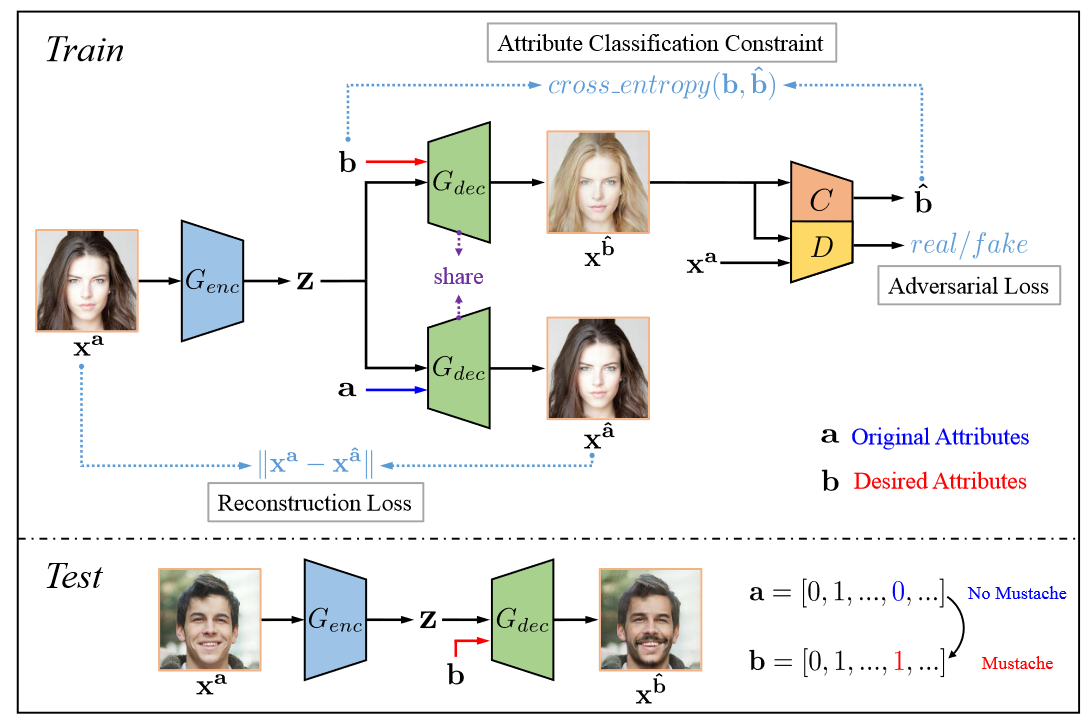
\includegraphics[width=0.8\textwidth]{images/attgan.png}
    \caption{Complete architecture of AttGAN.}
    \label{fig:attgan}
\end{figure}

\begin{figure}[H]
    \centering
    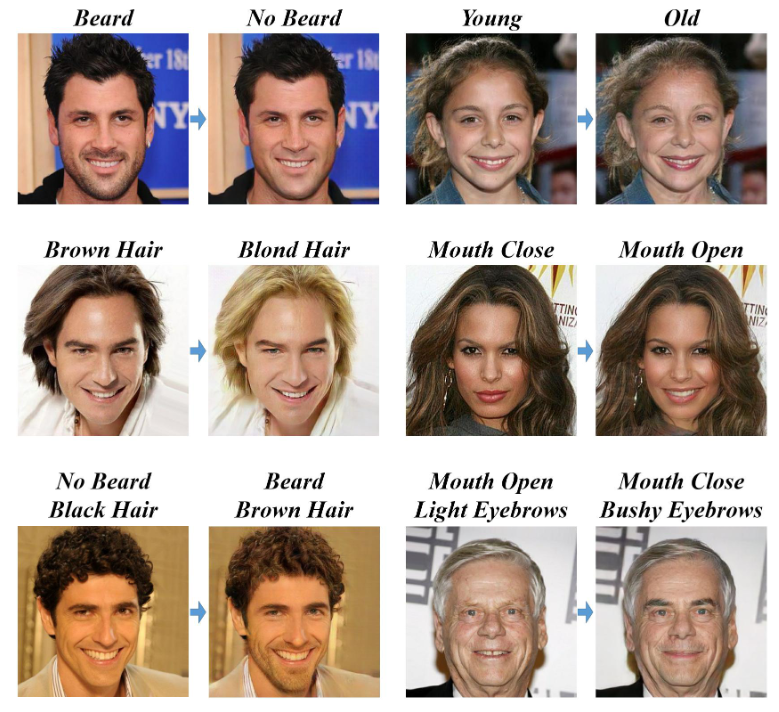
\includegraphics[width=0.8\textwidth]{images/attgan-results.png}
    \caption{Visual results of AttGAN.}
    \label{fig:attgan_res}
\end{figure}

\paragraph{InjectionGAN}
\texttt{InjectionGAN} \cite{9119402} uses the same concepts as AttGAN, but it has one more concept, which is using Feature-wise Linear Modulation (FiLM) layer which successfully infers information from external data and applies it as an affine transformation parameter to vision tasks, so they propose a new type of skip connection layers between encoder and decoder of the generator to add the new attributes shown in figure \ref{fig:injgan}. Visual results of InjectionGAN are shown in figure \ref{fig:injgan_res}

\begin{figure}[H]
    \centering
    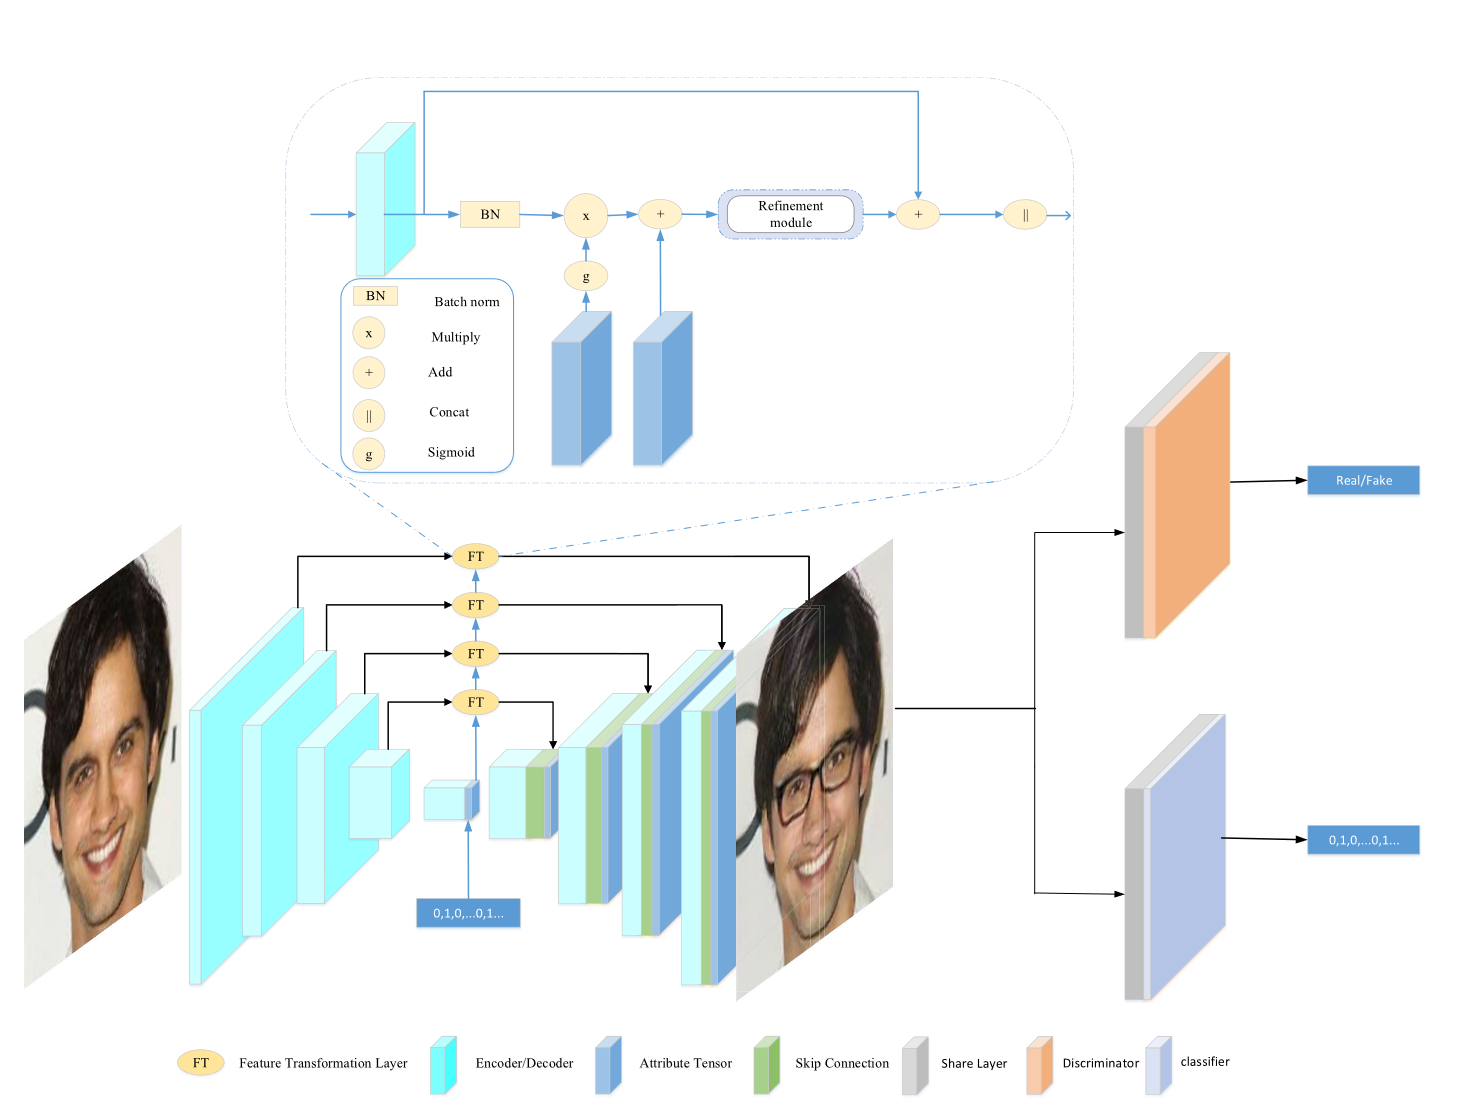
\includegraphics[width=0.8\textwidth]{images/injectiongan.png}
    \caption{Complete architecture of InjectionGAN.}
    \label{fig:injgan}
\end{figure}

\begin{figure}[H]
    \centering
    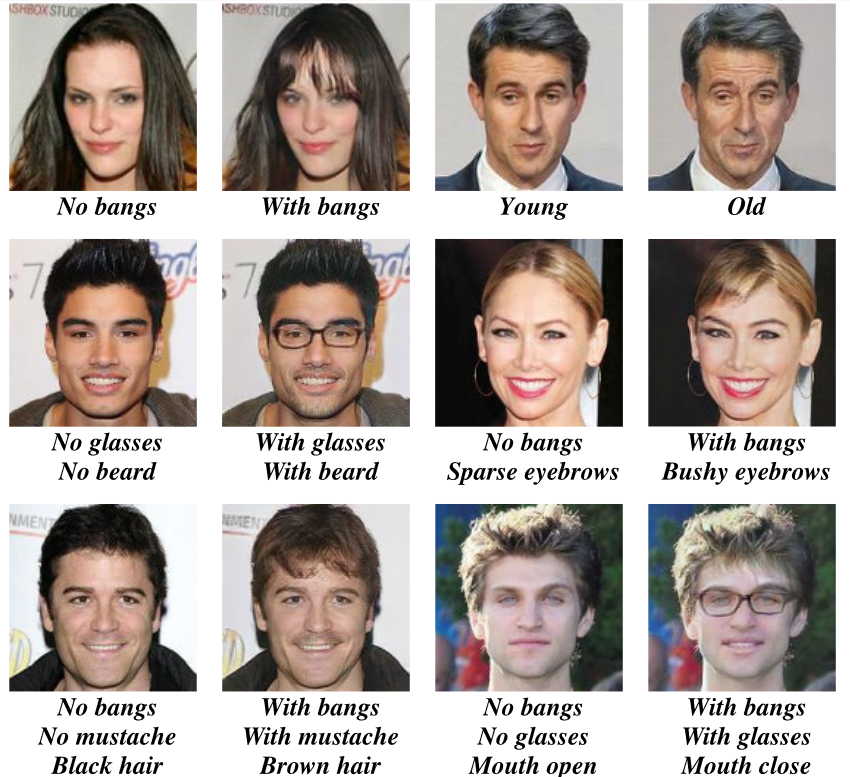
\includegraphics[width=0.8\textwidth]{images/injectiongan-results.png}
    \caption{Visual results of InjectionGAN.}
    \label{fig:injgan_res}
\end{figure}

\paragraph{Facelet-Bank for Fast Portrait Manipulation}
\texttt{Facelet Bank} \cite{chen2018faceletbank} follows the idea of navigation in GANs latent space, they added a new module called Facelet bank. It’s used as skip connections. It takes a bottleneck output from the decoder as input and passing it to a block of CNN layers and add it to the bottleneck output. This summation does the operation of the navigation in the latent space, so the Facelet layer should be trained to get the correct added value to different bottleneck outputs to  the same face with changing a specific attribute. Figure \ref{fig:facelet} shows the complete architecture, while figure \ref{fig:facelet_res} shows the visual results.

\begin{figure}[H]
    \centering
    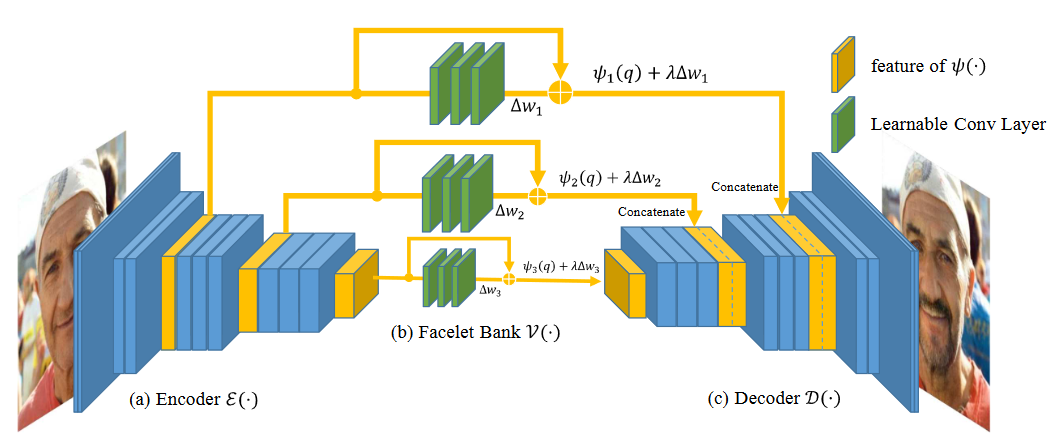
\includegraphics[width=0.8\textwidth]{images/facelet.png}
    \caption{Complete architecture of Facelet Bank.}
    \label{fig:facelet}
\end{figure}

\begin{figure}[H]
    \centering
    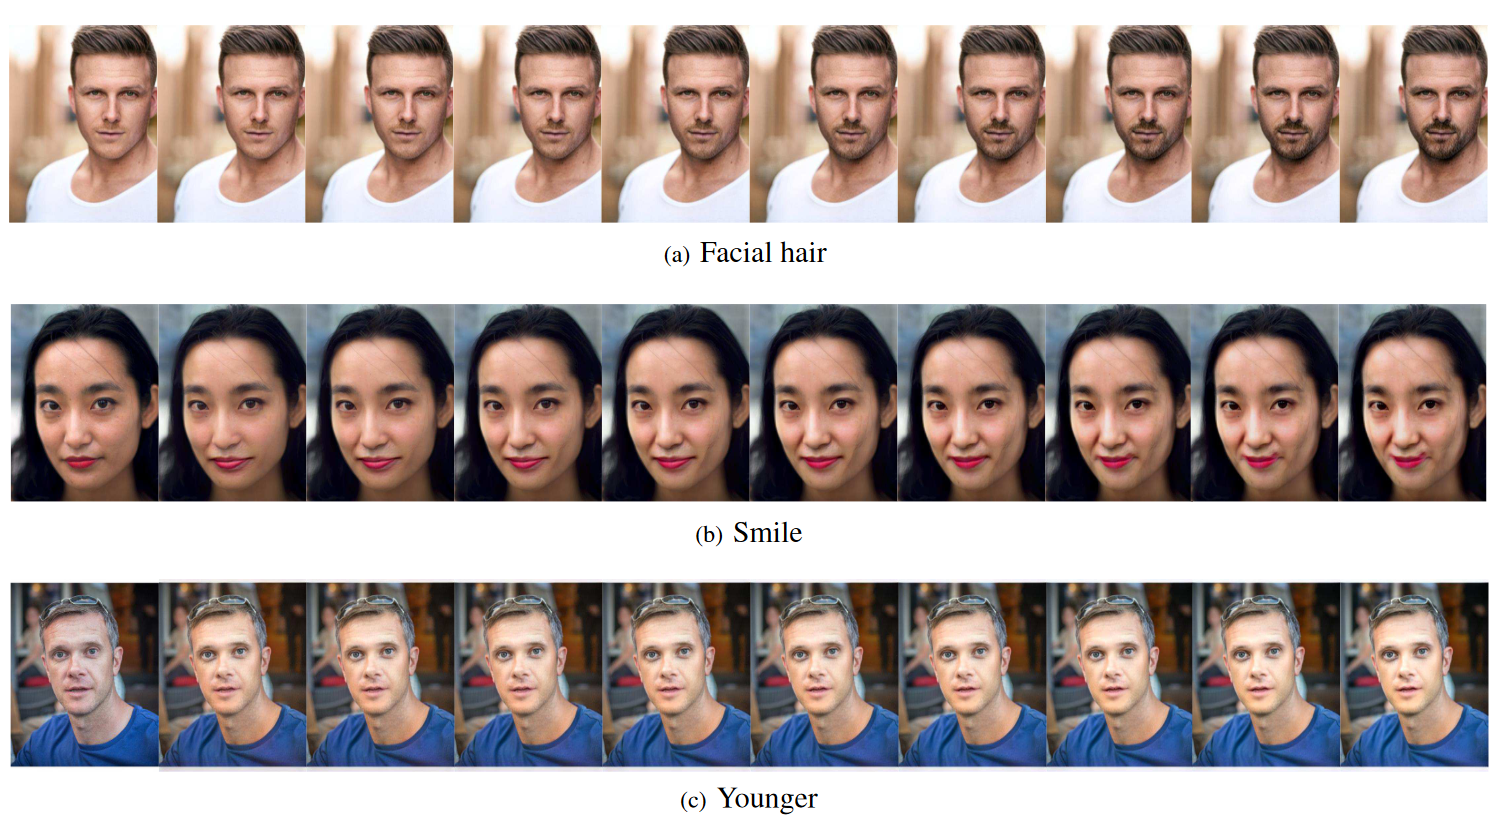
\includegraphics[width=0.8\textwidth]{images/facelet-results.png}
    \caption{Visual results of Facelet Bank.}
    \label{fig:facelet_res}
\end{figure}

\subsection{Face Rotation}
In this sub-section, we discuss different methods and approaches to generate multiple head poses from a single image. Note that, we focus on the methods that rotate a face, provided by a single image, with multiple angles of rotation, not just head frontalization. Also, the methods are ordered according to priority based on \emph{performance}, \emph{visual results} and \emph{involved work}.

\subsubsection{Rotate-and-Render}

\paragraph{Brief Description}
A DNN-based method under the title of \textbf{Rotate-and-Render: Unsupervised Photorealistic Face Rotation from Single-View Images} \cite{zhou2020rotateandrender}. The network is based on \emph{3D face modelling} with \emph{unsupervised deep learning}. 

\paragraph{Workflow}
It consists of three stages : 
\begin{itemize}
    \item \textbf{3D face fitting} which generates a 3D model of the face and extracts the face texture.
    \item \textbf{Rotate-and-render} which rotates the face in 3D space and renders it in different poses.
    \item \textbf{Render-to-image} which projects the 3D render of the face into a 2D image.
\end{itemize}
\textbf{Note :} The architecture, also, ensures \emph{cycle-consistency} through re-projecting the face into the initial pose.

\paragraph{Visual Results}
\begin{figure}[H]
    \centering
    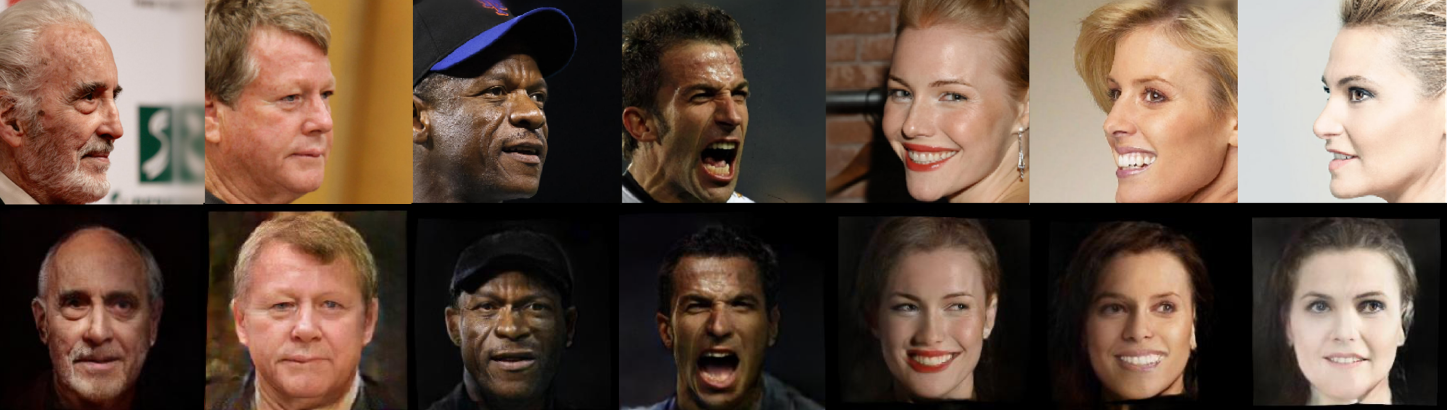
\includegraphics[width=\textwidth]{images/rotate-and-render.png}
    \caption{Visual results of Rotate-and-render network.}
    \label{fig:r&r}
\end{figure}

\subsubsection{DepthNets}

\paragraph{Brief Description}
A DNN-based method under the title of \textbf{Unsupervised Depth Estimation, 3D Face Rotation and Replacement} \cite{moniz2018unsupervised}. The network is based on \emph{casting} a specific face to a pose provided by another face in an \emph{unsupervised way}.

\paragraph{Workflow}
It consists of three stages :
\begin{itemize}
    \item \textbf{Landmark extraction} from both faces.
    \item \textbf{Image-to-image translation}.
    \item \textbf{Siamese-like architecture} that compares the generated face with the original one.
\end{itemize}

\paragraph{Visual Results}
\begin{figure}[H]
    \centering
    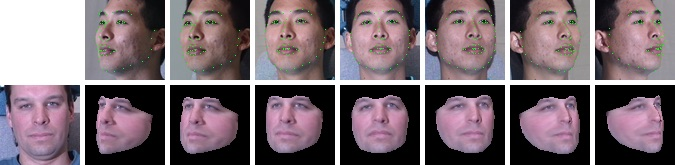
\includegraphics[width=\textwidth]{images/depthnets.png}
    \caption{Visual results of DepthNets.}
    \label{fig:dn}
\end{figure}

\subsubsection{PosIX-GAN}

\paragraph{Brief Description}
A DNN-based method under the title of \textbf{PosIX-GAN: Generating multiple poses using GAN for Pose-Invariant Face Recognition} \cite{inbook}. The network generates the provided faces in \emph{9 angles of rotation} in an \emph{end-to-end manner} that relies on datasets to train GANs.

\paragraph{Workflow}
It's an end-to-end network that depends on datasets for training.

\paragraph{Visual Results}
\begin{figure}[H]
    \centering
    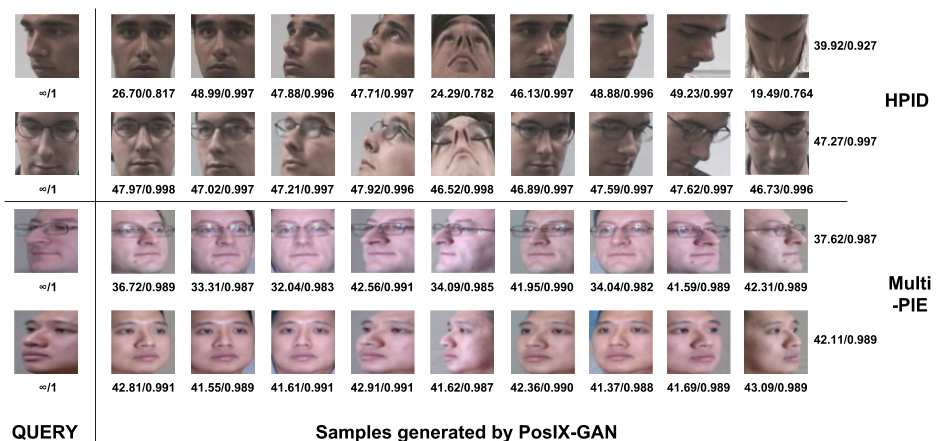
\includegraphics[width=0.8\textwidth]{images/posix-gan.png}
    \caption{Visual results of PosIX-GAN.}
    \label{fig:posix}
\end{figure}

\subsubsection{CAPG-GAN}

\paragraph{Brief Description}
A DNN-based method under the title of \textbf{Pose-Guided Photorealistic Face Rotation} \cite{8578974}. The network generates different head poses using a \emph{pose-conditioned generator} and \emph{couple-agent discriminator} that discriminates both identity and pose.

\paragraph{Workflow}
It's an end-to-end network that depends on datasets for training.

\paragraph{Visual Results}
\begin{figure}[H]
    \centering
    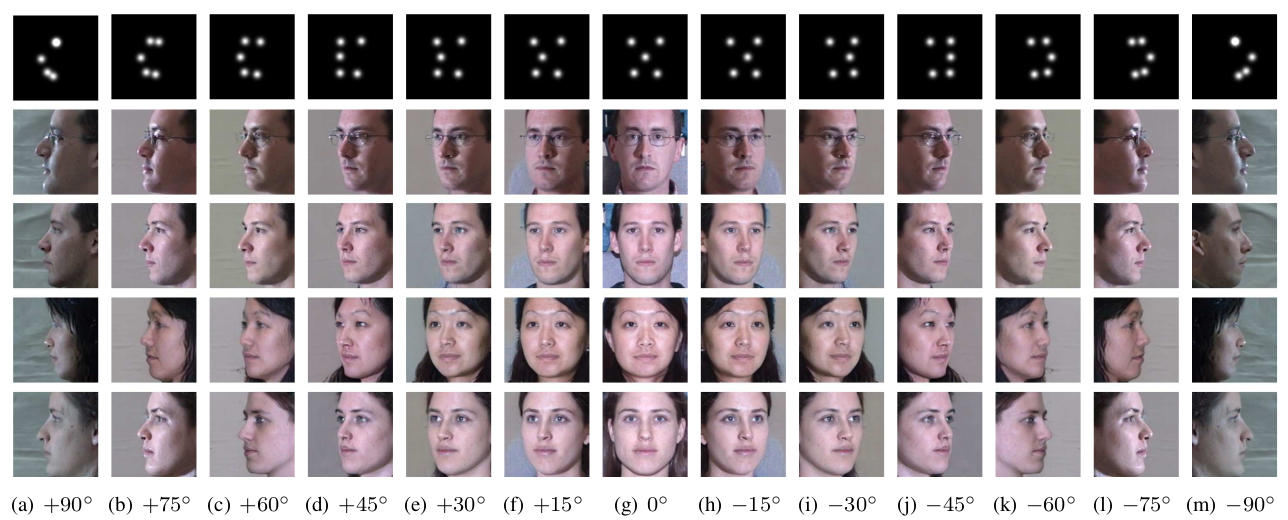
\includegraphics[width=\textwidth]{images/capg-gan.png}
    \caption{Visual results of CAPG-GAN.}
    \label{fig:capg}
\end{figure}

\subsection{Comparative Study of Previous Work}
From our previous discussion, we can see that \texttt{StyleGAN2} offers the best quality of faces, while being very flexible. The architecture is used in various research works related to image generation. Other approaches don't have the same flexibility and robustness. That's why we opted to use \texttt{StyleGAN2} as our main generative model. 

\texttt{Faces à la Carte} paper does not provide enough details about their method, as well. This is one of the reasons that encourages us to work on this project, in order to provide are clear pipeline for the problem solution.

Regarding face refinement, the most promising method is \texttt{Facelet Bank}, which can be used on high quality image. Also, the \emph{facelet bank} module is flexible enough to handle multiple facial features. However, in our final system, we chose not to go with this architecture for reasons, mentioned later in the document.

Finally, for face rotation, \texttt{Rotate-and-Render} and \texttt{DepthNets} offer an unsupervised framework for multiple face poses generation. This is better and much easier to adapt than other supervised methods, mainly because most of head poses datasets are not open-source. \texttt{Rotate-and-Render} can produce better visual results than \texttt{DepthNets}, because it can account for features such as hair through \emph{image inpainting} using \emph{image-to-image translation}. Overall, this yields better visual results.

\subsection{Implemented Approach}
Our system implements $3$ main functionalities, which are \textbf{text-to-face generation} (input can be \emph{speech} or \emph{text}), \textbf{face refinement} and \textbf{multiple head poses generation}. After extensive research and experimentation, we come up with our working pipeline that achieves our project goal.

\subsubsection{Face Generation from Description}
First of all, we start with our core and the most innovative part of our project. Face generation from bare description is very popular problem, yet few research works target it. To our knowledge, \texttt{Faces à la Carte} is the only available research paper that targets this problem. As we mentioned, the authors does not offer enough details about their method. Consequently, we have to utilize the related work to carefully design a fast and robust system for such problem. 
Our system can take different kinds of descriptions, including audio, text and manual inputs. That's why we have to create multiple stages of input processing and not to use direct end-to-end networks. 

The first processing stage is \emph{speech recognition}, which translates the speech into textual description. We opt to use \texttt{DeepSpeech2} \cite{amodei2015deep}, which is one of the most popular speech recognition architectures.

The second processing stage is \emph{text processing}, which converts the textual description into numerical attributes values. For this stage, we have many options, including classical and DL-based methods. However, we choose to work with \texttt{DistilBERT} \cite{sanh2020distilbert} due to multiple reasons. Basically, \texttt{DistilBERT} is a lightweight architecture that does not have a very big memory footprint. It's fast and easily tuned to our needs. Moreover, it does not use \emph{recurrent neural networks}, which are slow at inference time. Finally, we can adapt it to our desired output, which is not just classification, but the actual numerical values of the facial features.

The third and last processing stage is \emph{code generation}, which transforms the numerical attributes values into a face embedding that is used to guide the face generation process. This stage is completely designed from scratch and refined, iteratively, with face generative model (\texttt{StyleGAN2}). However, some previous research works are used for guidance, especially \texttt{Image2StyleGAN}, which guided our feature directions extraction process. However, our system considers more facial features than any of the previous works.

Finally, we come to the actual face generation model. For this, we opt to use \texttt{StyleGAN2}. The reason behind this choice is that \texttt{StyleGAN2} is the one of the most powerful image generators that produce high quality images. It's very flexible and can be adapted to many applications. Moreover, it does not required special hardware to be tuned, which is the case in \texttt{BigGAN} that requires \emph{Tensor Processing Units} (\emph{TPUs}).

\subsubsection{Face Refinement}
For the face refinement module, we choose to adapt our work in \textbf{face generation} to be used for refinement as well. This is mainly done to avoid including another model, which would have increased the memory footprint. Moreover, latent manipulation of \texttt{StyleGAN2} can offer better results than most face refinement architectures with more facial features to include. Consequently, \texttt{StyleGAN2} latent manipulation is considered for face refinement with an extended set of facial attributes to refine.

\subsubsection{Multiple Head Poses Generation}
Although it's possible to extract feature directions for the generated head poses for \texttt{StyleGAN2} as well, we don't consider using it for face rotation. This is mainly because face pose directions suffer from heavy entanglement with other features. Moreover, these directions don't preserve the face identity and can cause serious illumination problems. Consequently, we only keep this method as a backup plan. However, \texttt{Rotate-and-Render} is our main multiple head pose generation method. We used the same workflow to create our face rotation pipeline and integrate it to our system. The main reason behind choosing \texttt{Rotate-and-Render} is that the whole workflow can be decomposed into separate modules to can be edited and implemented to fit our needs. Also, it is an unsupervised architecture, which makes it easy to work with. Finally, it offers decent results compared to other architectures.


\newpage

\section{System Design and Architecture}
In this chapter, we discuss our working pipeline and system architecture in details.  Generally, our system takes a speech note, textual description or numerical attributes as an input. It processes the input description and outputs the initial human face portrait that corresponds to the given description. Afterwards, the user is allowed to manually control some facial attributes and morphological features and to rotate the face and render it in multiple poses. In the first section, we give an overview about the system. Then, we discuss the system architecture in the second section. In the subsequent sections, each module implementation is discussed in details.

\subsection{Overview and Assumptions}

As mentioned above, our system basically enables the user to describe a human face in words or using numerical values and turns it into a full human face portrait that can be manipulated and rendered in multiple poses. The system relies heavily on generative models and text processing, both are iteratively designed to obtain the required results. The overall flow can be described as follows :
\begin{itemize}
    \item The input speech notes are translated to text.
    \item The textual description (extracted from speech input or manually entered) is processed to extract the numerical values of the required facial features.
    \item The numerical values are used generate a face embedding vector that encodes the facial attributes in low dimensional space ($512D$).
    \item A generative model is specifically designed to translate from the low dimensional embedding into the full face portrait ($1024X1024$).
    \item The generated face portrait can be further refined by navigating the face embedding space and re-generating the face portrait.
    \item Once the user settles on the final face portrait, the system can render that face in multiple poses to provide further identification.
\end{itemize}

The previous flow provides a very versatile framework to generate face portrait and adjust it to your liking. However, there is an extremely large number of facial attributes and morphological features to describe a human face. Consequently, we have to choose a descriptive subset of these attributes to consider in the face description. We consider $32$ facial attributes for face description, which are listed as follows :
\begin{itemize}
    \item Overall face :
    \begin{itemize}
        \item Gender : Male / Female.
        \item Age : Young / Old.
        \item Thickness : Chubby / Slim.
        \item Shape : Oval / Circular.
        \item Skin Color : Black / White.
        \item Cheeks : Normal / Rosy.
    \end{itemize}
    \item Eyes :
    \begin{itemize}
        \item Color : Black / Blue / Green / Brown.
        \item Width : Wide / Narrow.
        \item Eyebrows : Light / Bushy.
        \item Bags Under Eyes : On / Off.
    \end{itemize}
    \item Nose :
    \begin{itemize}
        \item Size : Big / Small.
        \item Pointy : On / Off.
    \end{itemize}
    \item Ears :
    \begin{itemize}
        \item Size : Big / Small.
    \end{itemize}
    \item Jaw :
    \begin{itemize}
        \item Mouth Size : Big / Small.
        \item Lips Size : Big / Small.
        \item Cheekbones : Low / High.
        \item Double Chin : On / Off.
    \end{itemize}
    \item Hair :
    \begin{itemize}
        \item Color : Black / Blonde / Brown / Red / Gray.
        \item Length : Tall / Short.
        \item Style : Straight / Curly / Receding Hairline / Bald / with Bangs.
    \end{itemize}
    \item Facial Hair :
    \begin{itemize}
        \item Beard / None.
    \end{itemize}
    \item Race :
    \begin{itemize}
        \item White / Black / Asian.
    \end{itemize}
    \item Accessories :
    \begin{itemize}
        \item Glasses : Sight / Sun.
        \item Makeup : On / Off.
        \item Lipstick : On / Off.
    \end{itemize}
\end{itemize}

\subsection{System Architecture}

Now, let's discuss our system architecture. The system consists of $6$ modules, $3$ core modules of the project and $3$ auxiliary modules. These modules are deployed in a \emph{web application} to provide an easy-to-use interface for face generation and manipulation. Figure \ref{fig:system} shows the complete block diagram of the system architecture. Meanwhile, figure \ref{fig:app} shows the application design and how the modules are deployed in a web application. The \emph{core} modules are listed as follows :
\begin{itemize}
    \item \textbf{Text Processing :} processes the input textual description and extracts the corresponding numerical values of facial attributes. This problem is similar to \emph{multi-label text classification}, however the outputs are normalized scores of facial attributes, which are designed carefully to match the \emph{face code generation} process.
    \item \textbf{Face Generation :}
    \begin{itemize}
        \item \textbf{Code Generation :} converts the numerical attributes values to be low dimensional face embedding. This is the most \emph{important} and \emph{innovative} module of our system, because it glues the desired attributes scored with the latent space of the generative model (used to generate the face), resulting in more accurate quality outputs.
        \item \textbf{Code-to-Face Translation :} translates the low dimensional face embedding into the actual face portrait. For this purpose, we use \texttt{StyleGAN2}, which is a \emph{state-of-art latent-based generative model}, whose latent space can be manipulated easily to fit our needs.
    \end{itemize}
\end{itemize}

Meanwhile, the \emph{auxiliary} modules are listed as follows :
\begin{itemize}
    \item \textbf{Speech Recognition :} translates the input speech to textual description.
    \item \textbf{Face Refinement :} uses the same generative model to manually refine the generated face portrait through navigating the latent space.
    \item \textbf{Multiple Head Poses Generation :} rotates the generated face portrait and renders it into multiple poses.
\end{itemize}

We discuss each module in more details in the subsequent sections. Also, these modules are organized into a web application for easier usage, as shown in Figure \ref{fig:app}. The application is divided into :
\begin{itemize}
    \item\textbf{ Web (Frontend) :} which contains the user interface and, also, the \emph{speech recognizer}. The speech recognizer is moved to the frontend to reduce the network communication overhead between the web application and the server, as transmitting text is easier than transmitting speech. Moreover, the speech recognizer doesn't require high computational power, so it can be embedded in the web application.
    \item \textbf{Server (Backend) :} which is separated into two servers. First server contains the \emph{text processor} and the \emph{generative model} and serves the requests of face generation and refinement. Second server contains the \emph{pose generator} and serves the requests of face rotation.
\end{itemize}

\newpage

The two servers can communicate with each other to exchange the generated face portraits through \texttt{TCP sockets}. Meanwhile, the web application communicates and sends requests to the servers through \texttt{HTTP REST API}.

\subsubsection{Block Diagram}

\begin{figure}[H]
    \centering
    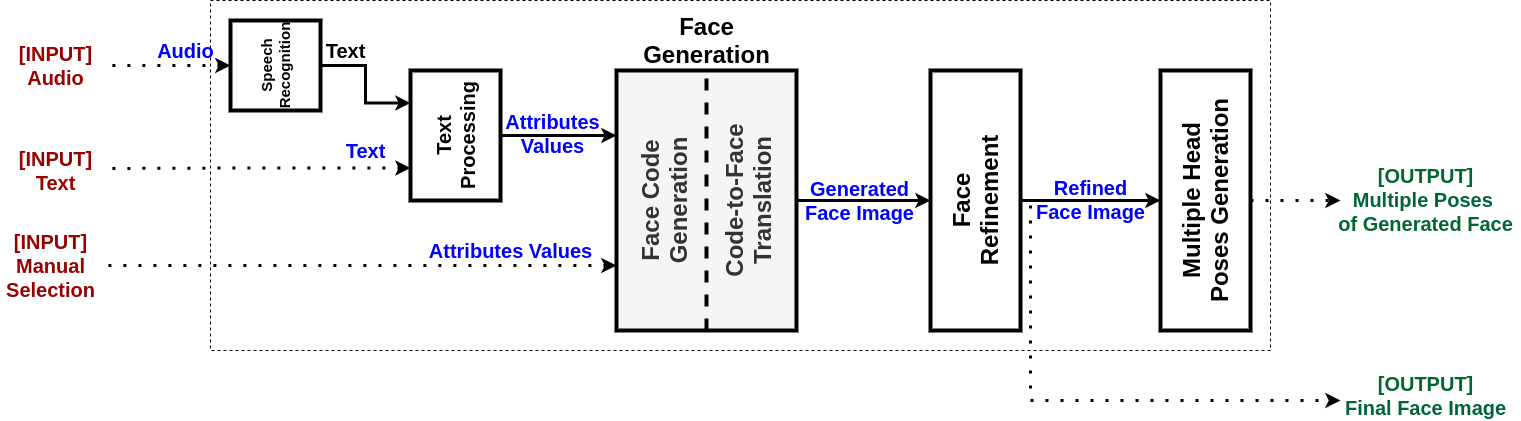
\includegraphics[width=\textwidth]{images/system-design.png}
    \caption{Block diagram of complete system architecture}
    \label{fig:system}
\end{figure}

\begin{figure}[H]
    \centering
    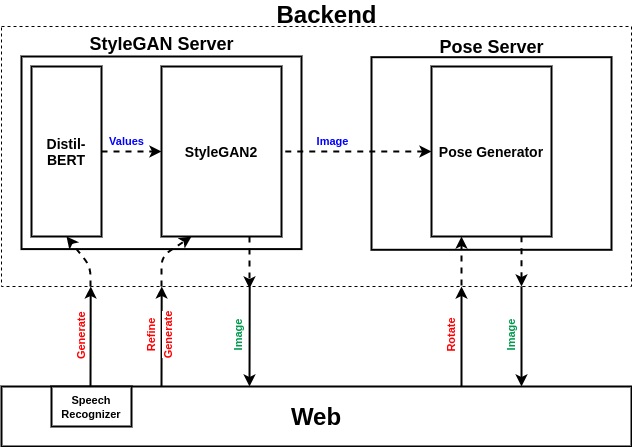
\includegraphics[width=0.8\textwidth]{images/app-design.png}
    \caption{Block diagram of application design}
    \label{fig:app}
\end{figure}

\subsection{Module 1 : Speech Recognition}
\label{sec:speech}
This is the first module in our pipeline, its responsibility is to get the textual description of the image from speech. It takes the speech as input then processes it to get its textual content to be used to extract the facial features used to generate the image.

\subsubsection{Functional Description}

Our aim is to add functionality that the user can enter a speech description of the image to generate it, so we used an automatic speech recognition model based on \texttt{DeepSpeech2} \cite{amodei2015deep}, we used the Spectograms features from the audio and applied some preprocessing to those features before training. The target of the speech model is to detect the English spoken words and get their textual meaning so that it can be used to generate the Face Image and output the desired described Face.

\begin{itemize}
    \item \textbf{Input :}
    \begin{itemize}
        \item Speech audio wave.
    \end{itemize}
    \item \textbf{Output :}
    \begin{itemize}
        \item The spoken words on the input audio (textual description).
    \end{itemize}
\end{itemize}

\subsubsection{Modular Decomposition}

\begin{figure}[H]
    \centering
    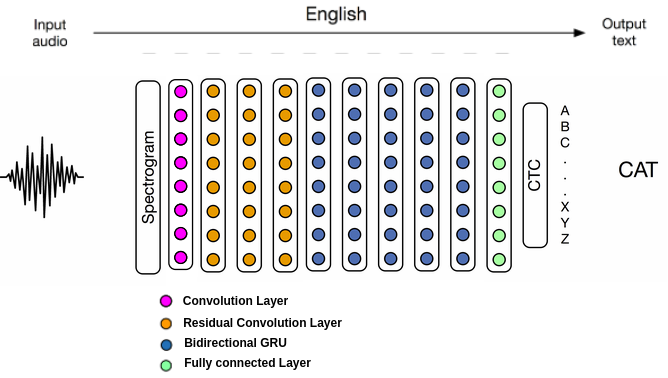
\includegraphics[width=0.8\textwidth]{images/speech.png}
    \caption{Modified DeepSpeech2 network architecture.}
    \label{fig:speechModel}
\end{figure}

As mentioned, we use \texttt{DeepSpeech2} with connectionist temporal classification (CTC) losses as a base to our speech recognition model. The model takes as input features from the audio in the form of spectrograms compressed by frequency and time masking to separate the spectrograms in time and frequency domains. \\
The model architecture (shown in figure \ref{fig:speechModel}) consists of one convolutional layer followed by 3 residual CNNs and 5 bidirectional gated recurrent units GRUs. \\

The first convolution layer used to compress the audio information in low dimension space, The residual CNN consists of layer normalization over the time axis of the speech then 2 convolution layers summed with the original input to the resCNN. \\

The bidirectional RNN uses 512 hidden units used to predict the input character at each time step, The last layer is a fully connected layer to out the final predicted character for each input spectrogram. \\

Connectionist Temporal Classification (CTC) loss function is used to align each character and its location in the audio input file, By summing the probabilities of possible alignments of the input to target and producing a loss value which is differentiable with respect to the model inputs and functions weights. After that those weights are updated using Adam optimizer to minimize this loss value until convergence. \\
\begin{equation}
    L(x,y;\theta) = - \log \sum_{l 	\in Align(x,y)}^{} \prod_{t}^{T} pctc (l_{t} |x;\theta )
\end{equation}

The best aligned character is selected using greedy beam search from all available character to the corresponding input. \\ 
The model Was trained and tested on LibriSpeech ASR corpus which consists of 100 hours for training and test set, "clean" speech for testing. We calculate the word error rate (WER) and character error rate (CER) for the test data to evaluate the model performance.


\subsubsection{Design Constraints}

As our application is a real time interactive app, It’s a must for the speech recognition model to be very fast to be able to process the input quickly so that we gain the users satisfaction. It was a constraint as we couldn't  use larger model with more accurate results, as it will increase the processing time which is against our needs.



\subsection{Module 2 : Text Processing}
\label{sec:text}
This module is the first stage in our pipeline that adds the feature of face generation from bare textual descriptions, not just manual manipulators. It's responsible for understanding the input textual description and converting it into facial features logits, where each logit describes how much the generated face should be saturated with. This task is done for 34 different facial attributes where each of them may or may not be entangled with other attributes, such as gender and beard attributes. Attributes may be on different levels as well, some of them are continuous, such as age, some are discrete, such as wearing sunglasses. see figure \ref{fig:scores_example} as an example. 

\begin{figure}[H]
        \centering
        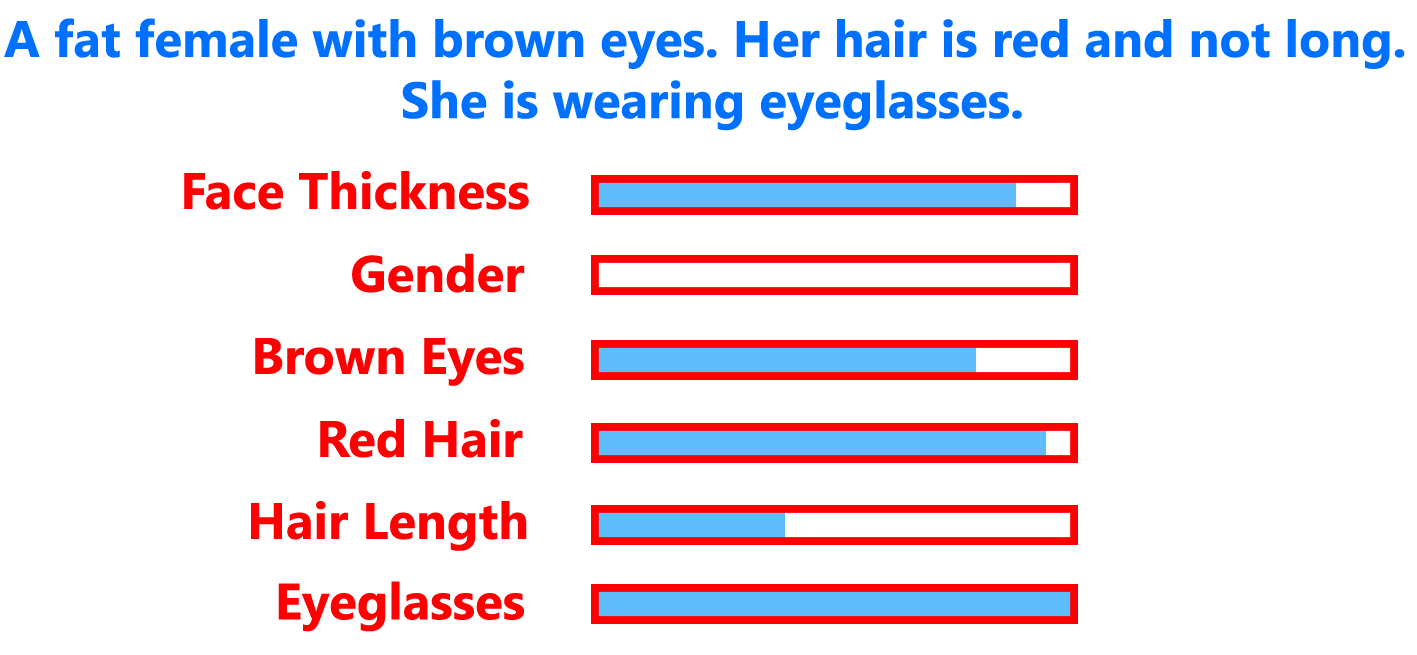
\includegraphics[width=0.8\textwidth]{images/scores-example.png}
        \caption{Attributes Scores Example}
        \label{fig:scores_example}
    \end{figure}


\subsubsection{Functional Description}
This module takes the input text and tries to 
\begin{enumerate}
    \item extract mentioned facial attributes.
    \item extract a score for each mentioned facial attribute referring to the level of saturation of this facial attribute.
    \item extract other non-mentioned attributes.
\end{enumerate}

Here’s the supported list of facial attributes that can be extracted:

\begin{itemize}

    \item Eyebrows
    \begin{itemize}
         \item Bushy Eyebrows               \hspace*{\fill Binary}
    \end{itemize}



    \item Hair Color
    \begin{itemize}
    	 \item Black Hair                   \hspace*{\fill Binary}
    	 \item Red Hair                     \hspace*{\fill Binary}
    	 \item Blonde Hair                  \hspace*{\fill Binary}
    	 \item Brown Hair                   \hspace*{\fill Binary}
    	 \item Gray Hair                    \hspace*{\fill Binary}
    \end{itemize}


    \item Hair Style
    \begin{itemize}
    	 \item Curly-Straight Hair          \hspace*{\fill Continuous}
    	 \item Receding Hairline            \hspace*{\fill Binary}
    	 \item Baldness                     \hspace*{\fill Binary}
    	 \item Bangs                        \hspace*{\fill Binary}
    	 \item Hair Length                  \hspace*{\fill Continuous}
    \end{itemize}


    \item Facial Hair
    \begin{itemize}
    	 \item Beard                        \hspace*{\fill Continuous}
    \end{itemize}


    \item Race
    \begin{itemize}
    	 \item Asian Race                   \hspace*{\fill Binary}
    	 \item Skin Color                   \hspace*{\fill Continuous}
    \end{itemize}


    \item General Facial Attributes
    \begin{itemize}
    	 \item Face Thickness               \hspace*{\fill Continuous}
    	 \item Gender                       \hspace*{\fill Binary}
    	 \item Age                          \hspace*{\fill Continuous}
    	 \item Lips Size                    \hspace*{\fill Continuous}
    	 \item Nose Size                    \hspace*{\fill Continuous}
    	 \item Ears Size                    \hspace*{\fill Continuous}
    	 \item Double Chin                  \hspace*{\fill Binary}
    	 \item High Cheekbones              \hspace*{\fill Binary}   
    	 \item Pointy Nose                  \hspace*{\fill Binary}
    	 \item Rosy Cheeks                  \hspace*{\fill Binary}
    \end{itemize}


    \item Eyes
    \begin{itemize}
    	 \item Black Eyes                   \hspace*{\fill Binary}
    	 \item Green Eyes                   \hspace*{\fill Binary}
    	 \item Blue Eyes                    \hspace*{\fill Binary}
    	 \item Brown Eyes                   \hspace*{\fill Binary}
    	 \item Eye Size                     \hspace*{\fill Continuous}
    	 \item Eye Bags                     \hspace*{\fill Binary}
    \end{itemize}


    \item Makeup
    \begin{itemize}
    	 \item Makeup Saturation            \hspace*{\fill Continuous}
    	 \item Lipstick                     \hspace*{\fill Binary}
    \end{itemize}


    \item Eyeglasses
    \begin{itemize}
    	 \item Sight Glasses                \hspace*{\fill Binary}
    	 \item Sun Glasses                  \hspace*{\fill Binary}
    \end{itemize}

\end{itemize}



\subsubsection{Modular Decomposition}
This module is considered as an NLP task that can be tackled using classical approaches, such as Text Parsing and Tagging, and Deep Learning approaches. The final design for this module is to use the power of Deep Learning approaches especially transformers to analyze and understand the text. This is because that the classical approaches failed in such a task as there are a lot of sequence dependencies on the textual description that may arise such as restricting the age of the described person to the range of low-to-medium beard levels and gender attribute, except in the case of age attribute is mentioned explicitly or implicitly in the text, for example "a boy", "a boy with a beard" and "a boy almost in his thirties", the first description should be understood as a child or teenager, while other descriptions refer to a middle-aged man. a lot of other dependencies that may arise that make the classical approaches not feasible and makes the deep learning solutions a must to tackle such a task. 
\\
\\
The biggest challenge in the Deep Learning approaches is that there are no available datasets mapping textual descriptions to facial features. That’s what led us to use synthesize our own dataset that must be much likely to be human-generated. This what made the module to be split into two sub-modules as shown in figure \ref{fig:text_processing_pipeline}. First one is the Dataset Synthesis sub-module and the Deep Learning Sequence Model to be trained on the synthesized dataset.


\begin{figure}[H]
        \centering
        
\includegraphics[width=0.8\textwidth]{images/text-processing-submodule.png}
        \caption{Text Processing Pipeline}
        \label{fig:text_processing_pipeline}
    \end{figure}

\paragraph{Dataset Synthesis sub-module}
This sub-module is the most critical one, as it should be as likely as possible to be human-generated. The approach we used to do so consists of three main stages as shown in figure \ref{fig:dataset_syn} in the reverse order of what needed in the training phase.

\begin{figure}[H]
        \centering
        
\includegraphics[width=0.8\textwidth]{images/data-synthesis.png}
        \caption{Dataset Synthesis Pipeline}
        \label{fig:dataset_syn}
    \end{figure}

\begin{enumerate}
    \item Random Attribute Generation
    
        In this stage, we generate any random attribute scores for all 34 attributes. Each attribute is generated with its pre-defined range of scores with one of random different modes
        
        \begin{itemize}
            \item Full Random Mode: All attributes will be mentioned in the text with random scores.
            
            \item Half-Length Random Mode: 50\% of attributes will be mentioned in the text with random scores, while other 50\% will not be mentioned.
            
            \item Short Random Mode: 20\% of attributes will be mentioned in the text with random scores, while other 80\% will not be mentioned.
            
            \item Very-Short Random Mode: 10\% of attributes will be mentioned in the text with random scores, while other 90\% will not be mentioned.
        \end{itemize}
        
        Mentioned Attributes are generated with some restrictions to make their scores consistent with others, such as
        \begin{itemize}
            \item Females, babies and children cannot have facial hair.
            \item Females cannot be bald.
            \item Males and babies cannot put makeup or lipstick.
            \item Bald people cannot have any hair attribute mentioned, such as hair color or hair style.
            \item One hair color at most can be mentioned (i.e. no person can have both yellow and red hair).
            \item One eye color at most can be mentioned (i.e. no person can have both blue and black eyes).
            \item People with bangs cannot have receding hairline and vice versa.
            \item One Eyeglasses type at most can be mentioned (i.e. no person wear both sun and sight glasses).
        \end{itemize}
    
    
    \item Random Textual Die Generation
    
    In this sub-module, a textual description is generated in a textual die using the random scores of facial attributes. Attributes are categorized using different categories, such as
    
    \begin{itemize}
    \item First Categorization is based on the facial part that is described, such as all hair attributes (Black Hair, Blonde Hair, Gray Hair, Red Hair, Brown Hair, Straight Hair, Hair Length) can be combined in a single description of the hair (e.g. a woman with long, brown and curly hair).
    \item Second Categorization is based on the grammatical way that the attribute can be described with. Each attribute can be of one or more of types below
        \begin{itemize}
            \item With Attributes: attributes that can be described using with statement (e.g. a man with brown hair and blue eyes.)
            \item Has Attributes: attributes that can be described using has statement (e.g. a man who has brown hair and blue eyes.)
            \item Puts Attributes: attributes that can be described using put statement (e.g. a woman is putting heavy makeup.)
            \item Wears Attributes: attributes that can be described using wear statement (e.g. a woman is wearing a glasses.)
            \item Full Statement Attributes: attributes that can be described using a full statement (e.g. His hair is brown. His Eyes is blue)
            \item Adjective Attributes: attributes that can be described using adjectives (e.g. a blond old man.)
        \end{itemize}    
    \end{itemize}
    
    Each mentioned attribute can have a form of different forms, such as
    \begin{itemize}
        \item Positive Attributes using Synonyms: describing an attribute with one of its synonyms randomly (e.g. “a man with a thick face.” can be described as a “a chubby man.”).
        \item Positive Attributes using Antonyms and Negation: describing an attribute with the negation of one of its antonyms randomly (e.g. “a man with a thick face.” can be described as a “He is not thin” or “a man with non-thin face.” and so forth).
        \item Negative Attributes using Antonyms: describing a negative attribute with one of its antonyms randomly (e.g. “a man with no thick face.” can be described as a “a thin man.”).
        \item Negative Attributes using Synonyms and Negation: describing a negative attribute with the negation of one of its synonyms randomly (e.g. “a man with no thick face.” can be described as a “He is not chubby” or “a man with non-thick face.” and so forth).
    \end{itemize}
    
    Each mentioned attribute chooses one of its categories and one of its forms randomly and reserve a slot in the textual die represented in figure \ref{fig:textual_die} .
    
    
    \begin{figure}[H]
        \centering
        
\includegraphics[width=0.8\textwidth]{images/textual-die.png}
        \caption{Textual Die where each attribute chooses a random slot for itself}
        \label{fig:textual_die}
    \end{figure}
    
    
    \item Paraphrasing
    
    
    As we use deep learning approaches, using the textual die to train a model is just making the model learn the die itself, not to generalize and extract the attributes from any other textual description. So, in this sub-module, we tried different approaches to restructure and paraphrase the textual die generated in the previous step, so that the generated description is more likely to be human-generated and to be general. To do so, we tried two approaches as a paraphraser
    
    \begin{itemize}
        \item First Approach: Training a Sequence-To-Sequence model using the “entailment” class in Stanford Natural Language Inference Dataset (SNLI) to re-structure any English statement to any other English statement based on the diversity of expressing ways in the English Language
        \item Second Approach: Using a random cycle of machine translators (e.g. translates the die in the sequence “English To Arabic To Spanish To Italian To English” or in the sequence “English To Chinese To English”). Using the power of different linguistic ways in different languages makes the paraphrased description more generic. 
    \end{itemize}
\end{enumerate}

\paragraph{Deep Learning Sequence Model}

The main task of Text Processing module is to map input textual description to corresponding attributes scores, so It’s a multi-class multi-label NLP problem. Therefore, in this sub-module we trained different deep learning architectures on the previously generated dataset. We tried 

\begin{itemize}
    \item LSTM Architecture: 2 BiLSTMs followed by a linear layer.
    \item Transformers Architecture: DistelBert-base-uncased, Bert-base-uncased, Albert-base-v2, Roberta-base
\end{itemize}

Where transformers architectures out-performed, so the final choice was DistelBert-base-uncased, as it’s the lightest one out of them with accuracy hit +99\% on validation.



\subsubsection{Design Constraints}
The design constraints of this module are enumerated as follows :
\begin{itemize}
    \item Human-like Dataset Synthesis: The biggest challenge of this module is that there’s no available dataset to tackle such a task. So, we needed to synthesize our own dataset that should be as generic and human-generated as possible, so that what made the paraphraser performance really matters.
    \item Conditional entailment of different facial attributes: as different facial attribute may affect each other, so the dataset should be generated in a robust way so that it can train the deep learning model to detect such relations, such as entanglement between beard, gender and age.
    \item Accuracy matters: as this is one of the early modules in the pipeline, the results of all other modules depend on its performance and accuracy. So, lack of accuracy in this module will be catastrophic for the whole pipeline.
\end{itemize}



\subsection{Module 3 : Face Code Generation}
\label{sec:code_gen}
Here, we discuss the face code generation from numerical values of facial attributes. This is the most important and innovative module in our system and the first stage of \emph{face generation}. It's worth \textbf{noting} that we use both of the terms \emph{"feature"} and \emph{"attribute"} to refer to a facial attribute, like hair color or nose size.

\begin{figure}[H]
    \centering
    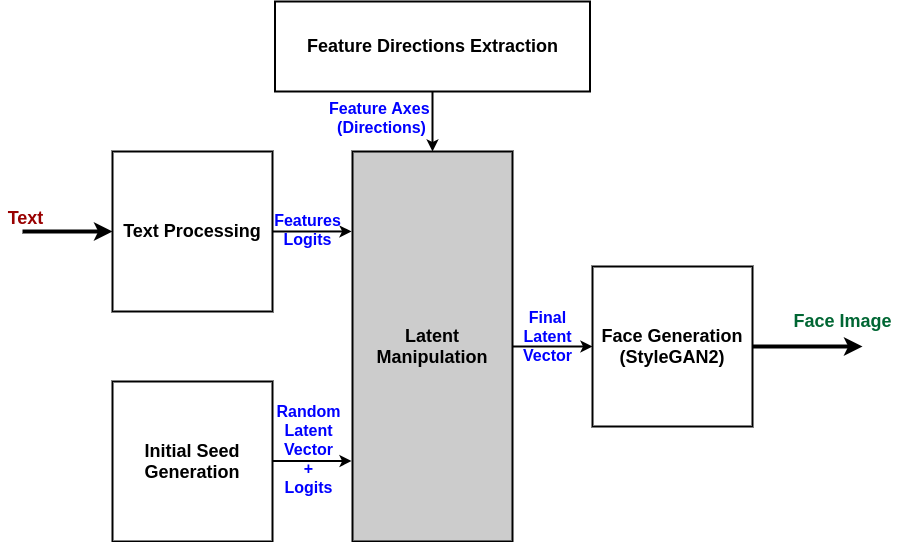
\includegraphics[width=0.8\textwidth]{images/face-gen-arch.png}
    \caption{Detailed block diagram of the three core modules workflow}
    \label{fig:face_gen}
\end{figure}

\subsubsection{Functional Description}

Figure \ref{fig:face_gen} shows a block diagram of the interaction between the $3$ core modules. We can see that the code generation module is the main driver of our face generation process. Generally, it converts the numerical attributes values (a.k.a. \emph{logits}) into a face embedding vector that matches the design of the latent space of the face generator (\emph{StyleGAN2}). Basically, it starts from an initial vector and uses the \emph{required feature values} and \emph{extracted feature directions} to transform this vector into the final latent vector, which is passed to the generative model.

\begin{itemize}
    \item \textbf{Input :}
    \begin{itemize}
        \item Numerical values of facial features (logits).
    \end{itemize}
    \item \textbf{Output :}
    \begin{itemize}
        \item Low dimensional face embedding vector (latent vector).
    \end{itemize}
\end{itemize}

\subsubsection{Modular Decomposition}

As figure \ref{fig:face_gen} tells, the code generation module can be torn down into $3$ sub-modules, which are \textbf{latent manipulation}, \textbf{initial seed generation} and \textbf{feature directions extraction}. Each sub-module is discussed in details to show how they integrate to each other to achieve the desired goal.

\paragraph{Feature Directions Generation}
Since, we use \texttt{StyleGAN2} \cite{karras2020analyzing} as our generative model, we have a full $512D$ latent space that is used to encode the whole face attributes. The changes in this latent space maps to the generated face image and similar features occupies the same area in the latent space. Consequently, we have to come up with a way to extract the axes (\emph{hyperplanes}) in this latent space to define each of our $32$ facial features. These feature directions are, then, used to manipulate the latent vector, in order to map to the required face image. 

\begin{figure}[H]
    \centering
    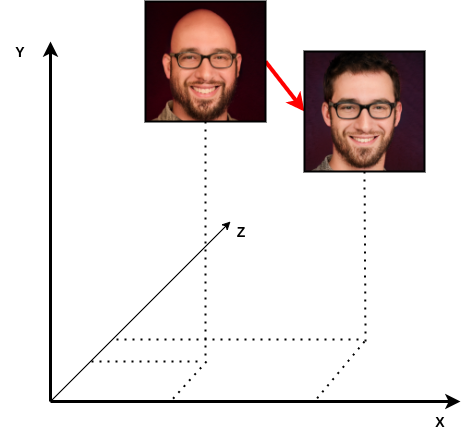
\includegraphics[width=0.5\textwidth]{images/feature-dir.png}
    \caption{Illustration of feature directions in latent space}
    \label{fig:feature_dir}
\end{figure}

Figure \ref{fig:feature_dir} further illustrates the idea of feature directions in the latent space. Here, we plot two face images in a $3D$ latent space. We can see that the difference between the two images in the existence and the absence of the hair, thus the red arrow represents the \emph{baldness} feature direction in that $3D$ latent space (moving along this particular vector causes hair density to change).

Our method of extracting the feature directions (\emph{hyperplanes}) consists of $3$ steps :
\begin{enumerate}
    \item \textbf{Code-Image Pairs Generation and Classification :} First, we use \texttt{StyleGAN2} to generate a large number of synthetic faces from random latent vectors. After so, we cluster the synthetic images (along with their latent vectors) according to each feature. The clustering can be based on discrete categories (like \emph{hair color} or \emph{race}) or continuous values (like \emph{hair length} or \emph{nose size}). We randomize the synthetic images in each clustering process to have better generalization and to cope with potential generation noise. For classification and regression, we use one of three possible methods, which are \textbf{manual labelling}, \textbf{classical image processing techniques} and \textbf{neural networks}. Thus, the output of this process is different groups of synthetic images sharing common facial features, along with their latent vectors.
    
    \item \textbf{Feature Directions Fitting :} Now, we have a set of latent vectors (\texttt{X}) and their corresponding feature values (\texttt{Y}). It's required to find a set of feature directions that satisfies the mapping between feature vectors and values. This problem can be formulated as :
    \begin{equation}
        Y = A_f \cdot X
    \end{equation}
    Where $A_f$ is the axis (direction) of feature $f$. \\
    We can obtain the solution to this equation in a closed form. However, due to the noise in both generation and classification, along with the non-linear nature of the problem, we opt to use \emph{ML} methods, specifically \textbf{Logistic Regression} and \textbf{SVM} to get an \emph{approximate solution}. Meanwhile, we cannot see any difference between the two methods, as they yield almost the same results. \\
    Finally, the generated feature directions are normalized to unit vectors :
    \begin{equation}
        A_{unit} = \frac{A}{||A||}
    \end{equation}
    
    \item \textbf{Directions Orthogonalization :} Facial features entanglement is one of the most difficult challenged of face generation. Some attributes in the human face tend to be extremely entangled by nature. For example, Asians rarely have curly hair, a woman cannot have beard and a man cannot put on makeup. Since \texttt{StyleGAN2} is trained and tuned on \textbf{FFHQ} dataset \cite{karras2019stylebased}, which contains real human faces, it is normal to notice some entanglement between some features. Consequently, the feature directions have to be further disentangled by using \emph{orthogonalization}. The orthogonalization process is done iteratively, starting from the most accurate feature directions. We orthogonalize other feature directions on the accurate ones, so that we have completely independent feature directions, where tuning one direction doesn't affect the others. The directions are orthogonalized as follows :
    \begin{equation}
        A_{proj} = (A \cdot B_{unit}) B_{unit}
    \end{equation}
    \begin{equation}
        A_{orthogonal} = A - A_{proj}
    \end{equation}
    
    Figure \ref{fig:ortho} visually illustrates the \emph{directions orthogonalization} process on $2D$ vectors.
    
    \begin{figure}[H]
        \centering
        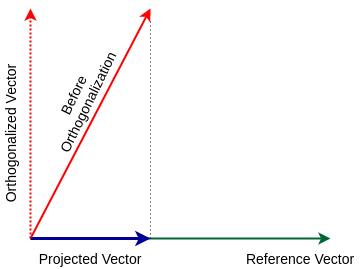
\includegraphics[width=0.5\textwidth]{images/orthogonalization.png}
        \caption{Illustration of orthogonalization relative to a reference vector}
        \label{fig:ortho}
    \end{figure}
    
    To ensure convergence to reasonable set of feature directions, we use a threshold margin to stop the orthogonalization process, which is from $85$ to $95$ degrees ($5$ degrees on each side of normal angle).
\end{enumerate}

\paragraph{Initial Seed Generation}
In order to avoid noise and discontinuities in the latent space, we generate an initial random latent vector. This is done by generating a random $512D$ vector and then passing it through the \emph{mapping network} of \texttt{StyleGAN2}, which is not invertible. This initial vector is, then, manipulated by sequential navigation along each feature direction (axis) with certain amounts. To get these amounts, we should know the component of the initial vector along each feature direction. We do that by simply performing a dot product between the initial vector and the unit vector of each feature direction. Thus, we have an initial latent vector and the numerical attributes values, it presents. 

\paragraph{Latent Manipulation}
This sub-module ingests all the inputs and produces the required latent vector (\emph{face embedding}) that describes all of the required facial attributes. The inputs to this latent manipulation sub-module are \emph{initial random vector} along with its logits, \emph{text logits} and \emph{feature directions}. The latent manipulation, simply, wants to realize the following transformation on the \emph{initial random vector} :
\begin{equation}
    E_{final} = E_{initial} + (l_{text} - l_{rand}) D
\end{equation}
Where $E_{final}$ is the final latent (\emph{embedding}) vector of dimensions $1X512$, $E_{initial}$ is the initial random vector of dimensions $1X512$, $l_{text}$ is the text logits vector of dimensions $1X32$ (remember that we consider $32$ facial features), $l_{rand}$ is the logits vector of the initial random vector of dimensions $1X32$ and $D$ is the feature directions matrix of dimensions $32X512$. The transformation includes calculating the difference between the required logits and the random logits and, then, use this difference to move the initial random vector along the feature directions to reach the final latent vector.

It might seem straight forward to perform this transformation. Unfortunately, it's not feasible to perform the transformation using direct matrix multiplication, mainly due to heavy \emph{entanglement} between direction vectors even after \emph{orthogonalization}. Also, the latent space of \texttt{StyleGAN2} can be very noisy in certain regions, so transformations have to be done carefully. 

Consequently, the processing in this sub-module is done iteratively as follows :
\begin{itemize}
    \item Both random and text logits are scaled from $0$ to $1$, which cannot have significant effect, when navigating using unit directions. Consequently, the inputs logits are scaled with the directions scale, which is obtained empirically to be from $-4$ to $4$, as shown in figure \ref{fig:dir_scale}.
    \item The next step is to get the \emph{difference} between \emph{text logits} and \emph{random logits}, which is of dimensions $1X32$. We call that \textbf{differentiated logits}. It's worth noting here that the input text usually contains a \emph{subset} of the facial features. Consequently, \emph{not all} the text logits are set to specific values. So, when doing the \emph{differentiation}, we set the differentiated logits of the \emph{unmentioned facial features} to $0$. So, it can be summarized as follows :
    \begin{equation}
        l_{diff}=
        \left\{ \begin{array}{ll}
            l_{text} - l_{rand} & l_{text} \neq None \\
            0 & \text{otherwise}
        \end{array} \right.
    \end{equation}
    \item Loop over each direction in feature directions :
    \begin{itemize}
        \item Multiply the \emph{differentiated logit} corresponding to the \emph{current feature} with its \emph{direction}.
        \item Add the product to the current latent vector (starting with the \emph{initial random vector}). The following equation summarizes these steps :
        \begin{equation}
            E_{next} = E_{prev} + l_{diff}[j] * D[j]
        \end{equation}
        \item Finally, to ensure that every transformation is independent of the subsequent transformations and that they are applied sequentially, we re-compute the \emph{produced latent vector logits} and re-differentiate it with the \emph{text logits}. This is done on every iteration of the latent manipulation process.
    \end{itemize}
\end{itemize}

\begin{figure}[H]
    \centering
    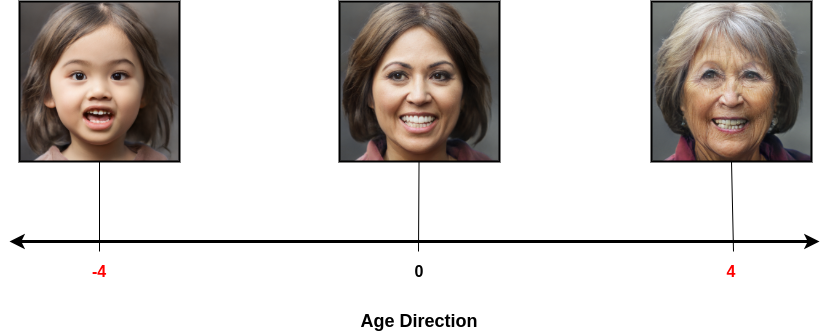
\includegraphics[width=0.8\textwidth]{images/dir-scale.png}
    \caption{Illustration of directions scale using age direction}
    \label{fig:dir_scale}
\end{figure}

By applying the previous process, the \emph{numerical value} of facial features extracted from text or manually entered by the user can be converted into a complete face embedding (\emph{latent vector}) matching the required facial attributes. This vector can be passed to \texttt{StyleGAN2} to translate it to a complete human face image.

\subsubsection{Design Constraints}

The design constraints of this module are enumerated as follows :
\begin{enumerate}
    \item \textbf{Facial attributes entanglement} is the main challenge of the face code generation module. Naturally, human face attributes are related to each other. For example, Asians barely have curly hair, no woman cannot have beard and most women have long hair and wear makeup. We mentioned before that \texttt{StyleGAN2} is trained and refined on \texttt{FFHQ} dataset, which contains real human faces. Consequently, it's normal to see heavy entanglement between features in the latent space. Due to this \emph{entanglement}, we have to perform extra computations to get decent results.
    \item \textbf{Random initialization} of the latent vector can cause some issues with the final output, as the vector can be initialized in a noisy area of the latent vector. We try to \emph{limit} the initialization of latent vector to a certain set of random vectors to avoid this effect. This method significantly reduces the \emph{random initialization effect}, however it's not fully cured.
    \item \textbf{Directions accuracy} can be a challenge as well. Some factors can negatively affect the feature directions accuracy. These factors include \textbf{synthetic image clustering} (whether \emph{classification} or \emph{regression}) and \textbf{directions fitting} process. We already discussed our solutions to this problem.
\end{enumerate}

\subsubsection{Synthetic Image Clustering}

As we mentioned before, it's required to cluster the generated synthetic images, in order to be able to fit the feature directions. The \emph{clustering} process can be performed through \emph{classification} or \emph{regression}. For example, features like hair and skin colors should be classified (grouped) into discrete categories, however features like hair length and mouth size should be assigned a continuous value. We do this task using one of three different methods :
\begin{enumerate}
    \item \textbf{Manual labelling} is the first idea to come to our minds. It's straight forward to manually classify a group of faces according to a certain feature. This method is used with some features, however it's very cumbersome and only works for classification.
    \item \textbf{Classical image processing techniques} are, also, used to classify images based on some features. Mainly, we use these techniques to detect \emph{colors} like eye color and hair color. We use \emph{morphological operators} and \emph{classical segmentation} to detect \emph{the eye} or \emph{the hair} and then retrieve its color.
    \item \textbf{Deep learning techniques} (\emph{neural networks)} are used to perform regression on the rest of the features. We basically use \emph{facial landmark detection} pretrained networks to detect the important facial landmarks, which is, then, used to calculate \emph{sizes} and \emph{distances}.
\end{enumerate}


\subsection{Module 4 : Code-to-Face Translation}
\label{sec:face_gen}
 Here, we discuss the process of converting the face embedding (\emph{latent vector}) to a complete face image using \texttt{StyleGAN2} (our chosen generative model). We discuss our reasons for choosing this particular architecture and how we use it.

\begin{figure}[H]
    \centering
    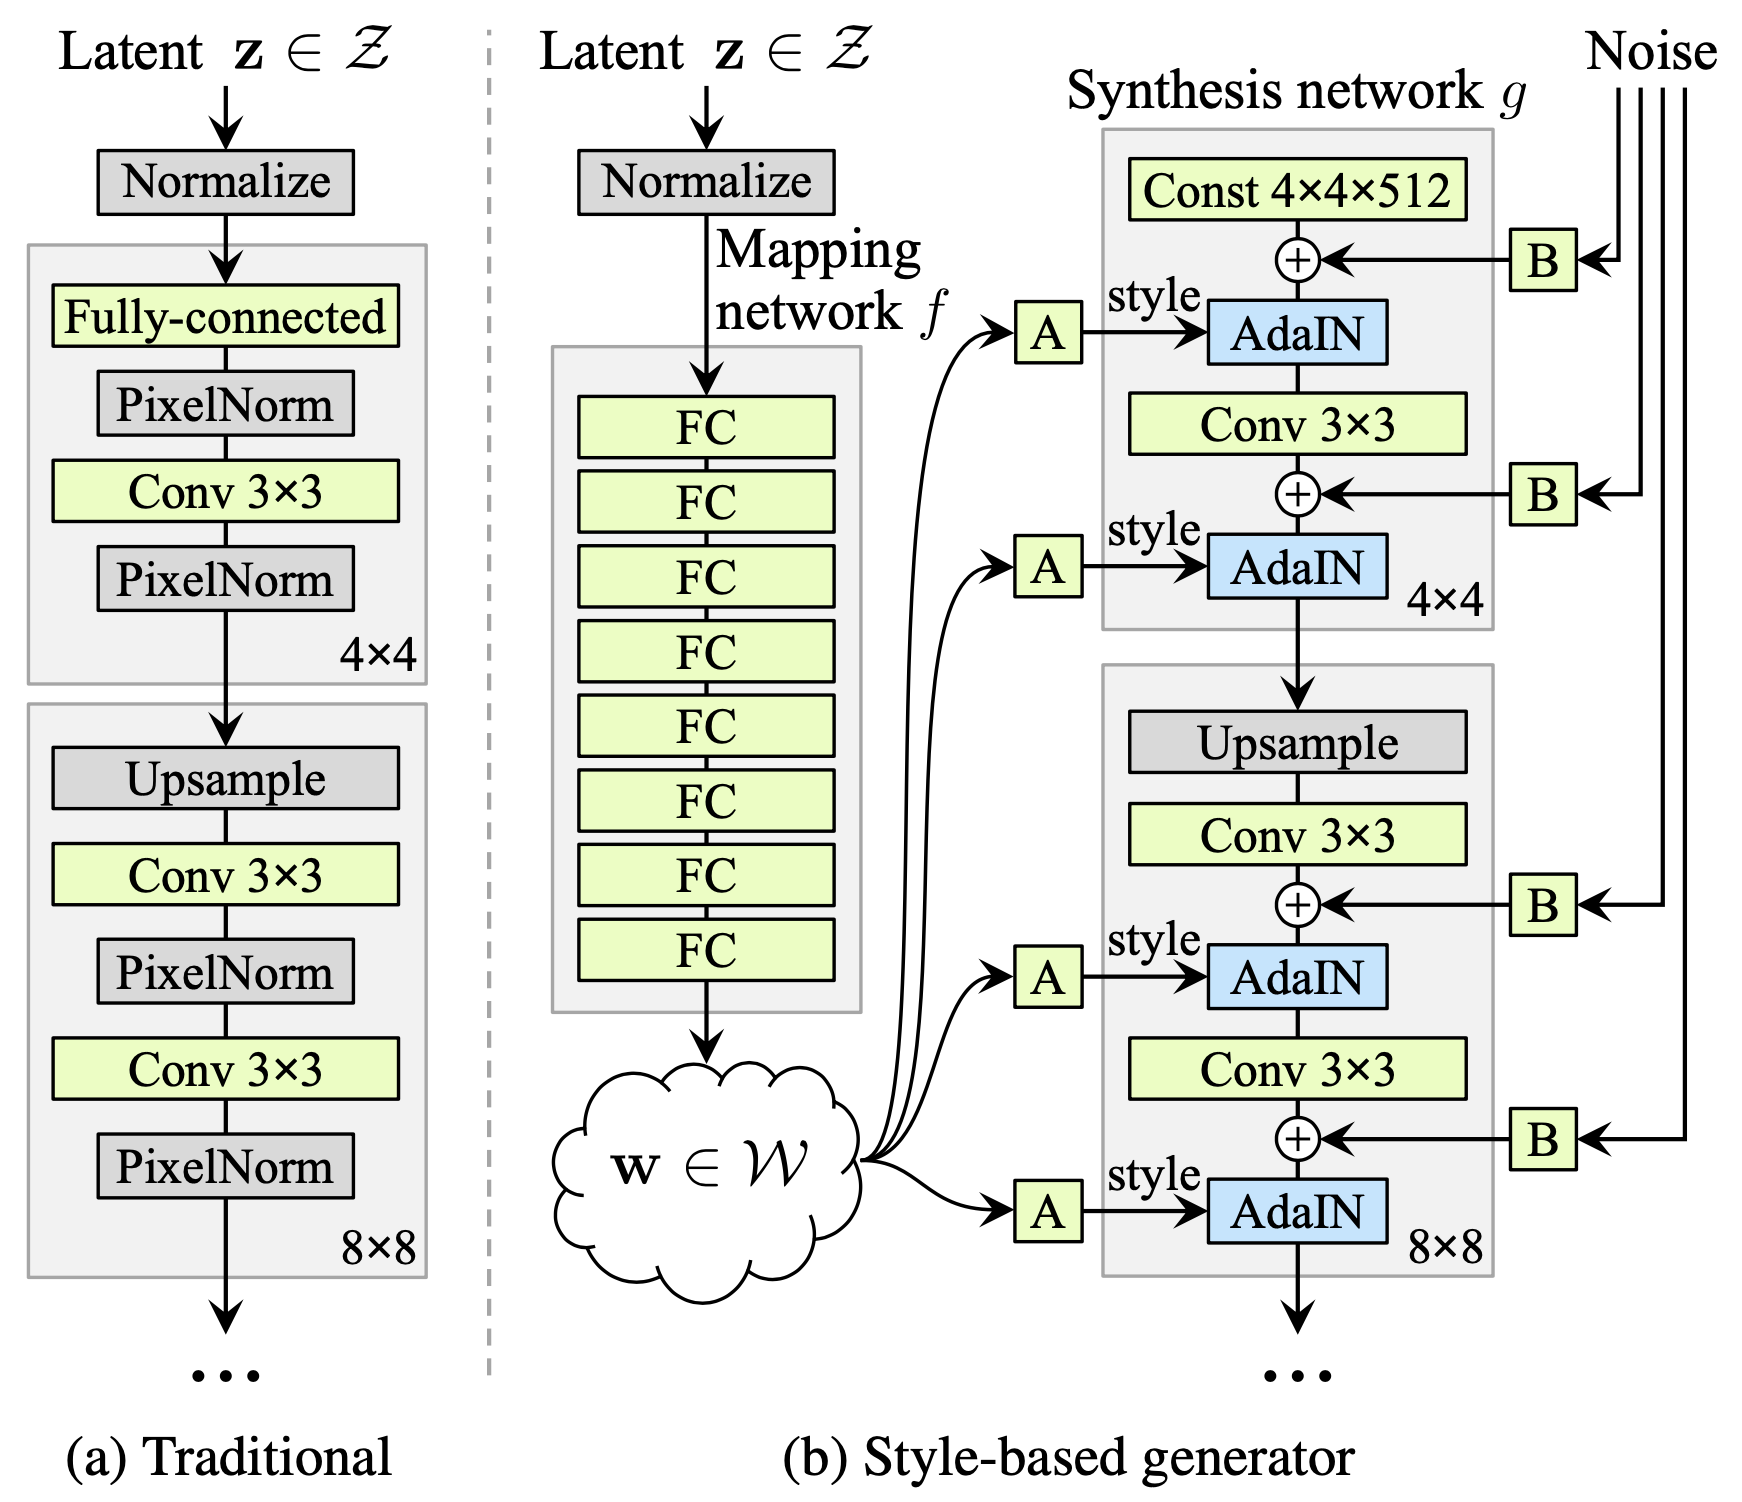
\includegraphics[width=0.7\textwidth]{images/stylegan.png}
    \caption{Style-based GAN architecture against traditional GAN}
    \label{fig:stylegan}
\end{figure}

\subsubsection{Functional Description}

This module utilizes the power of \emph{style-based} generative models, specifically \texttt{StyleGAN2} \cite{karras2020analyzing}, to translate the required \emph{latent vector} to a complete \emph{human face image}. \emph{Style-based GANs} (sometimes called \emph{latent-based GANs}) can exert artistic control over the generated content (images, videos, text ..., etc). Consequently, we can tune it to fit our need and, iteratively, design it along with \emph{code generation} \ref{sec:code_gen} and \emph{text processing} \ref{sec:text}, in order to have a complete end-to-end pipeline for \emph{text-to-face generation}.

\begin{itemize}
    \item \textbf{Input :}
    \begin{itemize}
        \item Low dimensional face embedding vector (latent vector).
    \end{itemize}
    \item \textbf{Output :}
    \begin{itemize}
        \item Complete human face image (portrait).
    \end{itemize}
\end{itemize}

\subsubsection{Modular Decomposition}

As mentioned before, we opt to use \emph{Style-based GANs} to be able to artistically control the output and designed the whole pipeline for \emph{text-to-face generation}. Moreover, we choose \texttt{StyleGAN2}, because it's one of the most popular and robust Style-based GANs in research literature. Also, it's relatively lightweight compared to other GANs used for the same purposes, but most importantly, \texttt{StyleGAN2} excels at human face generation based on latent space. Figure \ref{fig:stylegan} shows the original architecture of \texttt{StyleGAN} and how it is compared to traditional GANs. \texttt{StyleGAN} generator has two networks as follows :

\begin{itemize}
    \item \textbf{Mapping network} creates nonlinear transformation to the input latent vector $z$ ($512D$). This transformation is not invertible and results in a $512D$ latent vector $w$. This latent vector $w$ is expanded into several $512D$ vector using affine transformation, which gives the \emph{extended latent vector} $w+$. The extended latent vector $w+$ dimensions depend on the dimensions of the output image.
    \item \textbf{Synthesis network} generates the synthetic image from \emph{normally-distributed noise} guided by the extended latent vector $w+$.
\end{itemize}

\texttt{StyleGAN2} \cite{karras2020analyzing} is a newer version that follows the same architecture, but with some modifications to further improve the control over latent space and the quality of the outputs. 

So, let's discuss how we adapted \texttt{StyleGAN2} to our work :

\begin{itemize}
    \item To provide a high fidelity results, we target $1024X1024$ synthetic images. To achieve this, we have to use an extended latent vector $w+$ of dimensions $18X512$, meaning we repeat the latent vector $w$ $18$ times with \emph{affine transformation} for each.
    \item To further improve feature directions disentanglement, we fine-tune \texttt{StyleGAN2} using a subset of \texttt{FFHQ} dataset with increasing the weight of \emph{perceptual path regularization} in the loss function. \emph{Perceptual path regularization} in \texttt{StyleGAN2} loss encourages the smooth mapping between latent and image spaces. So, when increasing it in certain directions, it highly penalizes the deviation between latent and image spaces in these directions giving more organized latent space. To avoid using the whole dataset, we use \texttt{StyleGAN2} \emph{adaptive discriminator augmentation} (\textbf{ADA}) \cite{karras2020training} training methodology.
    \item Finally, we opt to remove the \emph{mapping network} of \emph{StyleGAN2} generator and only use the \emph{synthesis network}. This is mainly because :
    \begin{itemize}
        \item The mapping network doesn't satisfy the \emph{path length regularization}, so there is no smooth mapping between latent space $z$ and image space (only with latent space $w$). This is discussed in the original paper \cite{karras2020analyzing} and our experiments support that.
        \item The mapping network is not invertible, unlike the synthesis network. So, we cannot reverse the transformation from image space to latent space $z$. That's why we only work with latent space $w$ to test the consistency of the results.
        \item Removing the mapping network reduces the computations and the memory footprint, which is crucial in our case.
    \end{itemize}
\end{itemize}

After the previous modifications, the output model can directly translate the face embedding vector (\emph{latent space}) into a complete human face portrait. 

Notice that using this methodology of \textbf{code-to-face translation} along with \textbf{code generation} makes the sequential navigation in the latent space is \emph{easily invertible}, which eases the generation and the refinement (discussed in \ref{sec:face_ref}) of the synthetic face and gives the system versatility and fault tolerance. Figure \ref{fig:latent_nav} illustrates the idea of \emph{invertibility} of sequential edits on a $2D$ latent space example. Here, we show a simplified $2D$ latent space with $3$ feature direction. $AB$ vector represents the \emph{hair color} direction and $BC$ vector represents the \emph{gender} direction. Point $A$ starts with a \emph{blonde girl}, moving along $AB$ vector results in a \emph{girl with black hair} at point $B$. Then, moving along $BC$ vector gives us a \emph{man with black hair} at point $c$. Consequently, moving along $CA$ vector, which is the opposite of the resultant of $AB$ and $BC$, gives us the original face, thus inverting the sequential changes.

\begin{figure}[H]
    \centering
    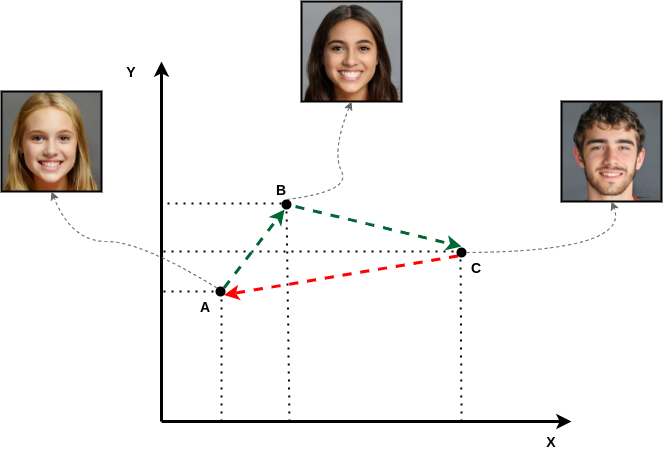
\includegraphics[width=0.7\textwidth]{images/latent-nav.png}
    \caption{Illustration of sequential navigation and invertibility in a $2D$ latent space}
    \label{fig:latent_nav}
\end{figure}

\subsubsection{Design Constraints}

The basic design constraints for this module can be enumerated as follows :

\begin{enumerate}
    \item \textbf{Network size} is surely one of our challenges. \texttt{StyleGAN2} has a large memory footprint, as the case with most \emph{deep generative models}. This constrains its training and deployment. We managed to remove the \emph{mapping network}, which gives us a change to use the full \emph{synthesis network}.
    \item \textbf{Faces dataset} is, also, a constraint, because real images of human faces contains entanglement between facial features (\emph{as discussed before}). So, we have to exert extra effort in the \textbf{code generation} module to solve some of this entanglement, emerging from real human faces datasets.
\end{enumerate}


\subsection{Module 5 : Face Refinement}
\label{sec:face_ref}
\subsubsection{Functional Description}

\subsubsection{Modular Decomposition}

\subsubsection{Design Constraints}

\subsubsection{Other Description}

\subsection{Module 6 : Multiple Head Poses Generation}
\label{sec:poses}
\subsubsection{Functional Description}

\subsubsection{Modular Decomposition}

\subsubsection{Design Constraints}

\subsubsection{Other Description}

\subsection{Other Approaches}
\label{sec:other_app}
At the beginning of our project, we tried to automate the whole pipeline in an \emph{end-to-end} deep learning approach starting from the textual input to the generated face. The pipeline is shown in figure \ref{fig:old}.

\begin{figure}[H]
    \centering
    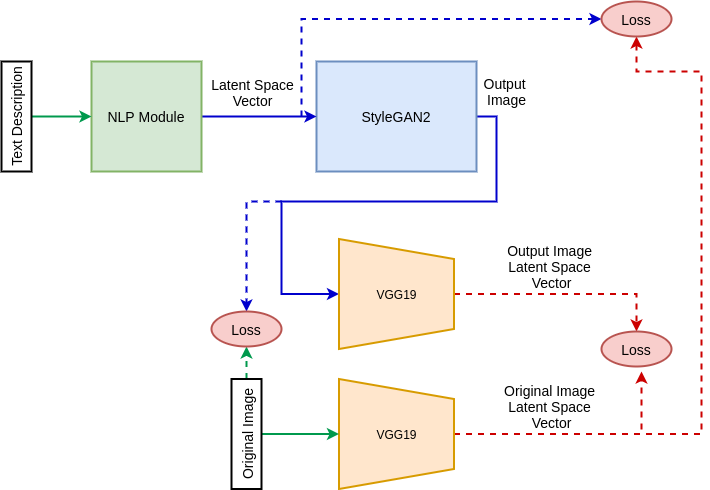
\includegraphics[width=0.7\textwidth]{images/old.png}
    \caption{Old Approach}
    \label{fig:old}
\end{figure}

\subsubsection{Face Generator Module}

We used the same latent-based generative model, which is \texttt{StyleGAN2} with no modifications. We aimed to use the generator pretrained weights to start the \emph{end-to-end} training process, which tunes the generator weights along with the whole system.

\subsubsection{NLP Module}

This module translates the text directly to the \texttt{StyleGAN2} latent vector $z$ that encodes all described facial features. We used a simple \emph{Recurrent Neural Network} (RNN) architecture that consists of $2$ recurrent layers followed by a fully connected layer. This is trained on a semi-synthesized dataset of text, latent vector and face image triplets.

\subsubsection{Dataset and Training}

Our dataset generation and the training process goes as follows :

\begin{itemize}
\item We started by using \emph{Face2Text} dataset that consists of $4000$ records of textual descriptions of images in the \emph{CelebA} dataset.
\item This dataset is very small, so we needed to make it larger :
\begin{itemize}
    \item We used \texttt{FaceNet} \cite{Schroff_2015} to encode the whole \emph{CelebA} dataset, as \texttt{FaceNet} is one of the best facial features extractors.
    \item We used \emph{K-Nearest Neighbors} (KNN) to get the closest $10$ matches of each celebrity in \emph{Face2Text} dataset from \emph{CelebA} dataset.
    \item Then, we manually picked the best $5$ matching faces out of the $10$ faces got from KNN. Therefore, we have a dataset of $20,000$ text-face pairs.
    \item We separately trained a strong feature extractor (\texttt{VGG19}) to map from face images to latent vector, which we called \emph{image-to-latent projector}.
    \item Finally, we used the image-to-latent projector to generate the latent vector corresponding to the dataset faces.
    \item Thus, we had the final dataset triplets of text, latent vector and face image.
\end{itemize}
\item Consequently, we trained our architecture \ref{fig:old} in an \emph{end-to-end} manner using the generated dataset. Mainly, we trained our NLP module and tuned \texttt{StyleGAN2} using a combined loss that consists of the summation of $3$ parts :
\begin{enumerate}
    \item Mean squared error (\emph{MSE}) loss between the output latent vector from NLP module and the project latent vector from the original image.
    \item Reconstruction loss between the output image from \texttt{StyleGAN2} generator using the output latent vector and the original image.
    \item Mean squared error (\emph{MSE}) loss between the projected latent vector of \texttt{StyleGAN2} generator output and the projected latent vector of the original image. This acts as a \emph{perceptual loss} and it's the most important part of our combined loss, as it ensures \emph{cycle consistency}.
\end{enumerate}
\end{itemize}

\subsubsection{Results}

Unfortunately, the previous architecture did not yield good results, due to many reasons :
\begin{itemize}
    \item The dataset was not robust and various enough to train such a huge network.
    \item We did not have enough computational resources to correctly and efficiently train this network for a long time.
    \item The latent space $z$ of \texttt{StyleGAN2} is very sensitive, so the NLP module has to be much more complex to be able to handle the latent vector generation. This was unfeasible given our resources.
\end{itemize}

Consequently, we opt to re-design our system in the staged manner, mentioned above, so that most of the system modules can use unsupervised learning or even no learning at all. 



\newpage

\section{System Testing and Verification}
In this chapter, we discuss how the system is tested both on module level and integration level. We discuss our \emph{performance metrics} and show the results of the system both \emph{quantitatively} and \emph{qualitatively}. We, also, show how our system performs compared to the baselines. Finally, we include the complexity analysis of our system for both time and memory.

\subsection{Testing Setup}

The testing environment of the whole system is basically targeting $4$ main properties :
\begin{enumerate}
    \item The quality of the output face images compared to the real human face images.
    \item The ability of the system to capture the included facial features in the input description and how they actually map to the output.
    \item The smooth and consistent mapping between the edits, imposed on the input description, and the changes of the output face image.
    \item The Independence (\emph{disentanglement}) between the different facial features.
\end{enumerate}

We create our testing strategy to assess these $4$ properties on the output face images. Also, we compare our results against the following baselines :

\begin{itemize}
    \item \texttt{StyleGAN2} \cite{karras2020analyzing} : We compare our results with the original \emph{StyleGAN2} to check the output quality.
    \item \texttt{Faces à la Carte} \cite{wang2020faces} : This is the only previous research work that attempted \emph{Text-to-Face Generation}.
    \item \texttt{Image2StyleGAN} \cite{abdal2019image2stylegan} : Our feature directions extraction methodology is inspired by this work, which is based on the first version of \emph{StyleGAN}.
\end{itemize}

\subsection{Testing Plan and Strategy}

To assess the $4$ previously-mentioned properties, multiple metrics are used, which are listed as follows :
\begin{enumerate}
    \item \textbf{Fréchet Inception Distance} (\emph{FID}) \cite{heusel2018gans} : This metric is an improvement over the traditional \emph{inception score} to be able to measure the similarities between a set of real and synthetic images. Basically, \emph{inception score} measures the ability of \texttt{Inception V3} network \cite{szegedy2014going} to classify a synthetic image into $1000$ classes. However, \emph{FID} measures the distance between synthetic and real images. This is done by extracting $2048D$ feature vector from each image using the \texttt{Inception V3} network and then calculating the \emph{Fréchet} distance using :
    \begin{equation}
        d^2 = ||\textbf{u}_{1} - \textbf{u}_{2}||^2 + Trace(\textbf{C}_{1} + \textbf{C}_{2} - 2 * \sqrt{\textbf{C}_{1} * \textbf{C}_{2}})
    \end{equation}
    Where $\textbf{u}$ is the feature-wise mean vector and $\textbf{C}$ is the covariance matrix of the feature vector.
    
    \item \textbf{Learned Perceptual Image Patch Similarity} (\emph{LPIPS}) \cite{zhang2018unreasonable} : This metric measures the smoothness of the mapping between the latent space edits and the output image changes. This metric takes as an input, two synthetic images. It uses a pretrained neural network to project them to a latent space. Then, it calculates the difference between the two latent vectors, along with the perceptual distance between the two images. Finally, it uses the two distances to calculate the final score. This metric is used in \texttt{StyleGAN2} paper to assess the \emph{perceptual path length}.
    
    \item \textbf{Edit Consistency Score} : We use this metric to ensure that the final facial attributes values are consistent with the input values after the \emph{latent manipulation} process. This metric is simply calculated by projecting the final latent vector over all feature directions and compare it to the input values.
    
    \item \textbf{Directions Disentanglement Score} : The disentanglement between feature directions are assessed by using the \emph{angles} between each pairs of directions. Angles of values $85$ to $95$ degrees usually indicates low entanglement. The angles between two directions is calculated by taking the \emph{inverse cosine} of the dot product between their unit vectors :
    \begin{equation}
        \theta_{1,2} = arccos(d1_{unit} \cdot d2_{unit})
    \end{equation}
\end{enumerate}

\subsubsection{Module Testing}

\paragraph{Speech Recognition}
Our final speech module is tested on \emph{LibriSpeech ASR} corpus, \emph{test-clean-speech} dataset. We use \emph{character error rate} (CER) and \emph{word error rate} (WER) to evaluate the accuracy of the model after $30$ epoch of training. Table \ref{tab:speech_results} show the results of our model.
\begin{table}[ht]
\centering
\caption{Speech recognition results.}
\begin{tabular}[t]{| c | c |}
\hline
CER & 0.25 \\
\hline
WER & 0.65 \\
\hline
CTC Losses & 0.7 \\
\hline
\end{tabular}
\label{tab:speech_results}
\end{table}

\paragraph{Text Processing}
Our Final Design for Text Processing module is considered as a multi-label multi-class classification using DistelBERT base uncased, so we finetuned then tested it on  a testing dataset of 100,000 records based on the metrics shown in table \ref{tab:text_metrics}. The metrics proved that it will work very well (almost perfect) in inference time.

\begin{table}[ht]
\centering
\caption{DistelBERT Testing Metrics.}
\begin{tabular}[t]{| c | c |}
\hline
Metric & Value \\
\hline \hline
Accuracy & 0.995 \\
\hline
Precision & 0.988 \\
\hline
Recall & 0.991\\
\hline
F1-Score & 0.989 \\
\hline
\end{tabular}
\label{tab:text_metrics}
\end{table}

\begin{table}[ht]
\centering
\caption{Runtime for different architectures.}
\begin{tabular}[t]{| c | c |}
\hline
Architecture & Runtime \\
\hline \hline
DistelBERT & 0.0072 sec \\
\hline
ALBERT & 0.0143 sec \\
\hline
BERT-base-uncased & 0.0127 sec \\
\hline
ROBERTA-base & 0.0125 sec \\
\hline
\end{tabular}
\label{tab:text_runtime}
\end{table}

We tried different architectures such as ALBERT, BERT-base-uncased, ROBERTA-base. All of them converged on almost the same metrics mentioned above from DistelBERT. On the other hand, DistelBERT is the lightest out of them as shown in table \ref{tab:text_runtime} of average runtime. So, DistelBERT was the optimal choice to use.

\paragraph{Code Generation}
To test the quality of the generated feature directions that are used for \emph{code generation}. We use two methods, which are \textbf{directions disentanglement scores} and \textbf{visual result} of moving along directions.

Table \ref{tab:angles} shows the angles between the directions of a subset of features. Remember that angles in range $85$ to $95$ degrees indicate low entanglement. Consequently, we can infer that the number, provided by the table, are reasonable. For example, the angle between \emph{gray hair} and \emph{age} directions is $79.6$ degrees, because old people normally have gray hair. Also, men are \emph{not} likely to wear makeup, so the angle between \emph{makeup} and \emph{gender} directions is $107.7$ degrees, same for \emph{beard} with men.

Moreover, figure \ref{fig:dir_results} shows the \emph{visual results} of moving along some feature directions. We use these results to qualitatively measure the accuracy of the extracted feature directions.

\begin{table}[ht]
\caption{Angles (measured in degrees) between different feature directions using a subset of the considered facial features (closer to $90$ degrees is better).}
\centering
\begin{tabular}[t]{| c | c | c | c | c |}
\hline
\textbf{Angles} & Age & Gender & Beard & Gray Hair \\
\hline \hline
Age & 0.0 & 92.4 & 85.8 & 79.6 \\
\hline
Gender & 92.4 & 0.0 & 80.0 & 88.6 \\
\hline
Makeup & 88.0 & 107.7 & 100.5 & 94.5 \\
\hline
Hair Length & 89.7 & 95.9 & 90.6 & 96.6 \\
\hline
\end{tabular}

\label{tab:angles}
\end{table}

\begin{figure}[H]
    \centering
    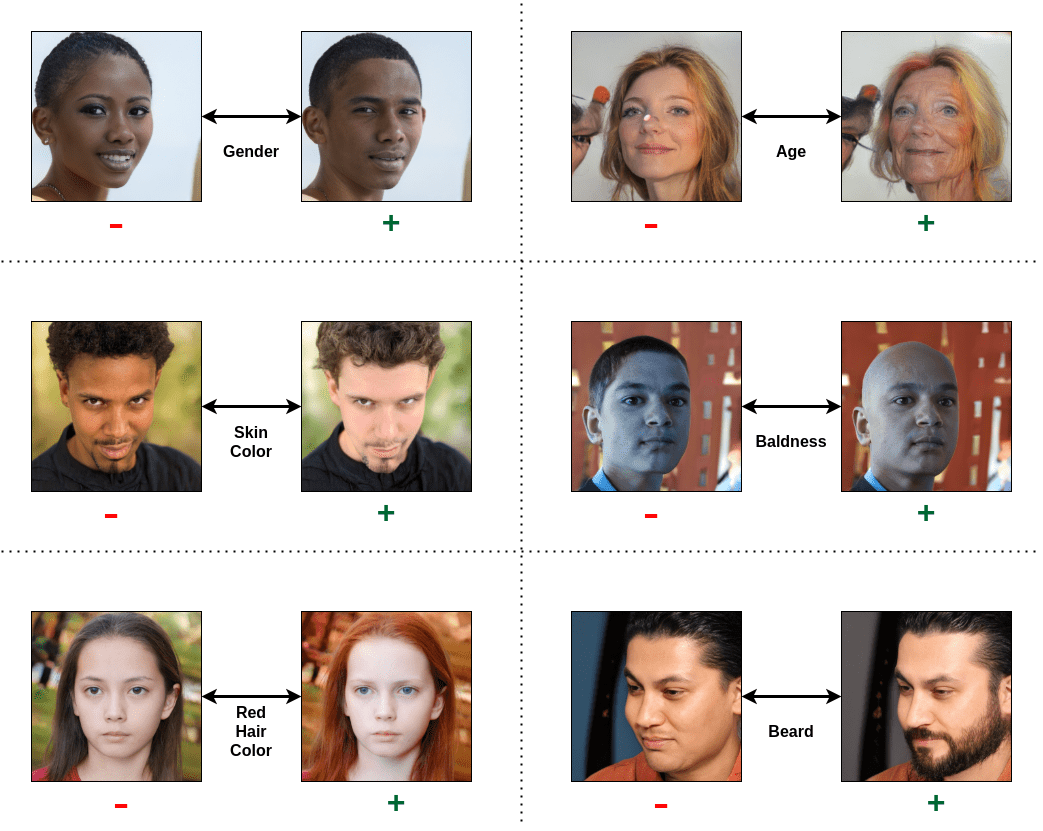
\includegraphics[width=\textwidth]{images/directions-results.png}
    \caption{The results of moving along some extracted feature directions.}
    \label{fig:dir_results}
\end{figure}

\paragraph{Code-to-Face Translation}
This module is basically tested using integration with \textbf{code generation}, which is shown in the \textbf{integration} test. However, we perform testing on this module separately using \textbf{edit consistency score} of the facial attributes values of the output image and the input values. 

As figure \ref{fig:edit_cons} shows, the system can convert a random vector (\emph{on the left}) to the final latent vector (\emph{on the right}) driven by the input values (\emph{on top}). Also, we can see the consistency between the required values and the values corresponding to the generated face.

Also, table \ref{tab:lpips} shows the relation between \emph{LPIPS} score (between the intial and output images) and the number of directions, navigated during face generation. We can see that the score increases, as the number of navigated directions increases. This is mainly because the output face image is far from the initial face image. However, we can see that some \emph{anomalies} can occur, like the case of the input text \emph{"Woman with lipstick and rosy cheeks"}, which navigates along only $3$ directions, but gives a high \emph{LPIPS} score.

\begin{figure}[H]
    \centering
    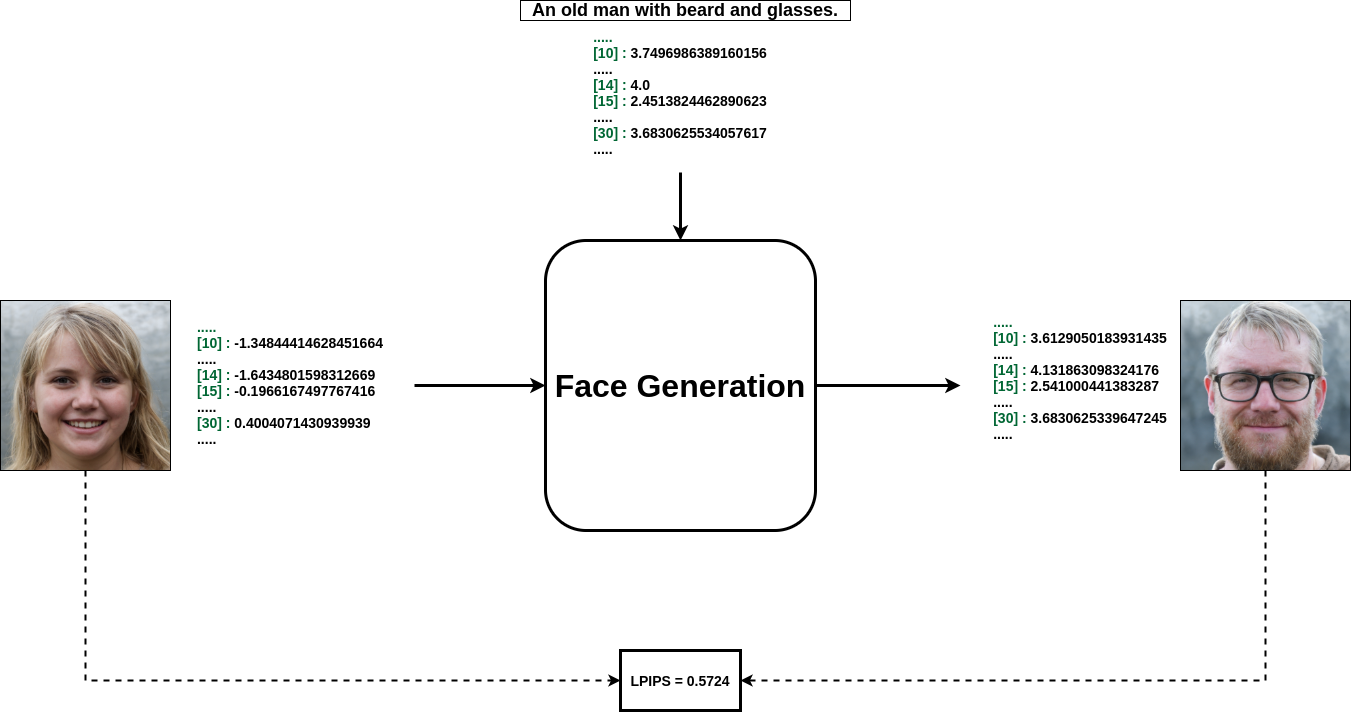
\includegraphics[width=\textwidth]{images/edit-consistency.png}
    \caption{An example of the consistency in reaching the required facial attributes starting from initial random vector.}
    \label{fig:edit_cons}
\end{figure}

\begin{table}[ht]
\centering
\caption{LPIPS values against the number of navigated directions for sample text (lower is better).}
\begin{tabular}[t]{| c | c | c |}
\hline
Input Text & Number of Navigated Directions & LPIPS \\
\hline \hline
Female with chubby face & 2 & 0.3905 \\
\hline
Woman with long wavy hair & 3 & 0.4412 \\
\hline
Old black man with glasses & 4 & 0.5023 \\ 
\hline
Woman with lipstick and rosy cheeks & 3 & 0.5107 \\
\hline
Young black man with long hair and beard  & 5 & 0.5733 \\
\hline
Old man with chubby face and glasses & 4 & 0.4905 \\
\hline
\end{tabular}
\label{tab:lpips}
\end{table}

\paragraph{Face Refinement}
Since, we adapt \texttt{StyleGAN2} for the refinement process, so this module testing is almost the same as \textbf{code-to-face generation} module. However, we focus more on the visuals of the \emph{sequential navigation}, along with the new features related to the face morphology. Figure \ref{fig:nav_res} shows the results of sequential navigation given an original synthetic face image. We tried to maintain the independence of sequential direction navigation as much as possible to keep the results visually acceptable. For example, in the first row, we convert from a \emph{"young man with hear and no beard"} into an \emph{"old bald man with beard"} by sequential navigation using \emph{age}, \emph{beard} and \emph{baldness} directions. This yields much better visual results than many recent \emph{attribute-editing GANs}.

\begin{figure}[H]
    \centering
    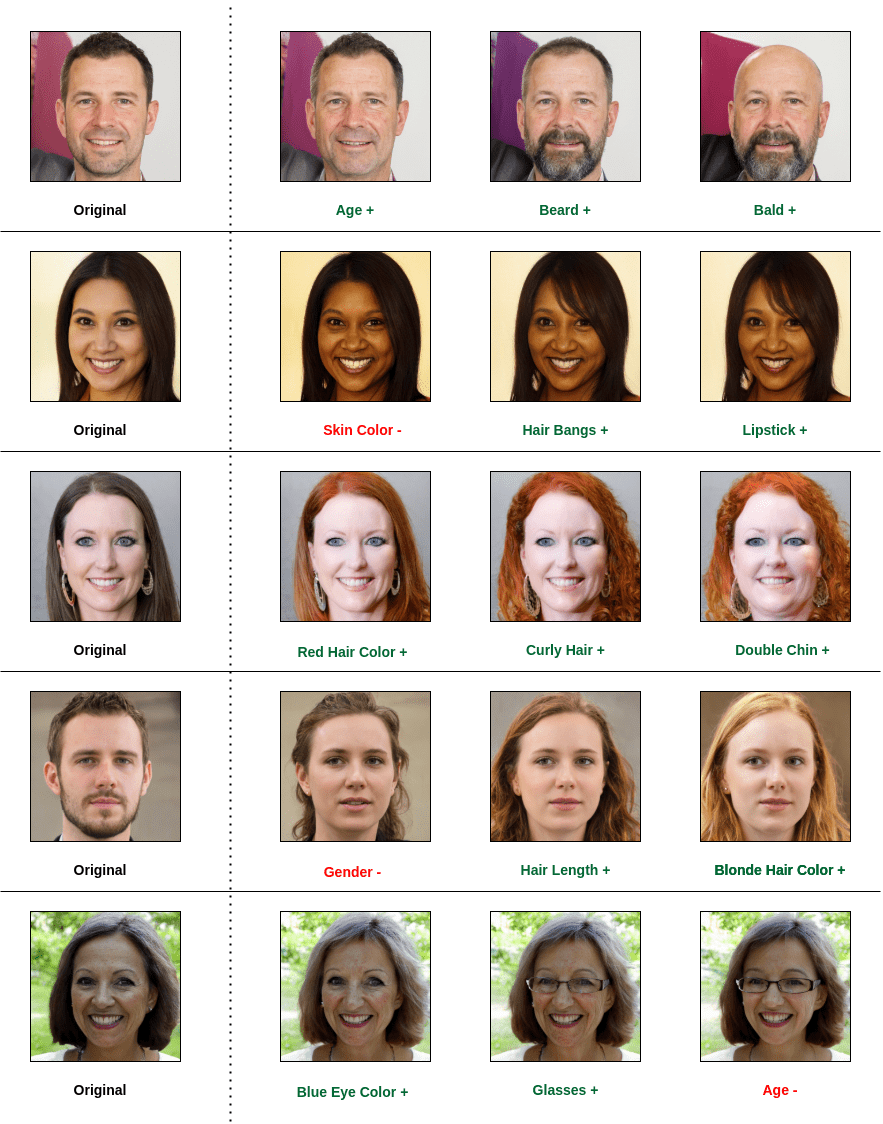
\includegraphics[width=\textwidth]{images/sequential-nav.png}
    \caption{The results of sequential navigation along certain feature directions.}
    \label{fig:nav_res}
\end{figure}

\paragraph{Multiple Head Poses Generation}

In order to test the Multiple Head Pose Generation module, 2 Tests are performed : \\

\begin{table}[H]
\caption{NME mean and std for test data of AFLW and AFLW2000 dataset. NME is calculated for a various range of poses for 3DMMs}
\centering
\begin{tabular}[t]{| c | c | c |}
\hline
Pose Range & NME on \textbf{AFLW} & NME on \textbf{AFLW2000} \\
\hline \hline
[0-30] & 7.65±5.41 & 5.668±2.88 \\
\hline
[30-60] & 9.11±6.47 & 7.05±4.04 \\
\hline
[30-90] & 10.04±8.33 & 8.28±4.42 \\
\hline
\textbf{[0-90]} & \textbf{8.93±0.98} & \textbf{7.002±1.06} \\
\hline
\end{tabular}
\label{nme_table}
\end{table}

\begin{itemize}
    \item \textbf{Quantitative Testing}: Calculating a metric on a Dataset to evaluate the performance of the 3D Fitting sub-module. The dataset used are AFLW (21 annotated facial landmarks) and AFLW2000 (68 annotated facial landmarks) datasets which contains Human faces and their corresponding Parameters for the 3DMM. The used metric is the Normalized Mean Error (NME) which is the standard metric for evaluating 3D Fitting models. NME is calculated for the single 3DMM as follows: \\
    
    \[ NME = \frac{1}{N} \sum_{k=1}^{N}\frac{l2norm(x _{k} - y _{k})}{d}\]
    
    Where d is the distance in the 3D model between the 2 eyes of the face. Results of NME metric are reported in table \ref{nme_table}

    \item \textbf{Qualitative Testing}: In addition to the Quantitative evaluation for the module, A Quantitative evaluation is performed by generating and visually evaluating results for Images outputted from our previous modules. Doing this asserts that the generated images have a user-friendly quality and doesn't mess up with the quality of the image generated in the previous steps. In figure \ref{fig:input_pose} we provide an example of some input face images generated from the previous modules. Qualitative results for the 3 input examples are displayed in figure \ref{fig:pose_output1}, figure \ref{fig:pose_output2}, figure \ref{fig:pose_output3}
    
    \begin{figure}[H]
    \centering
    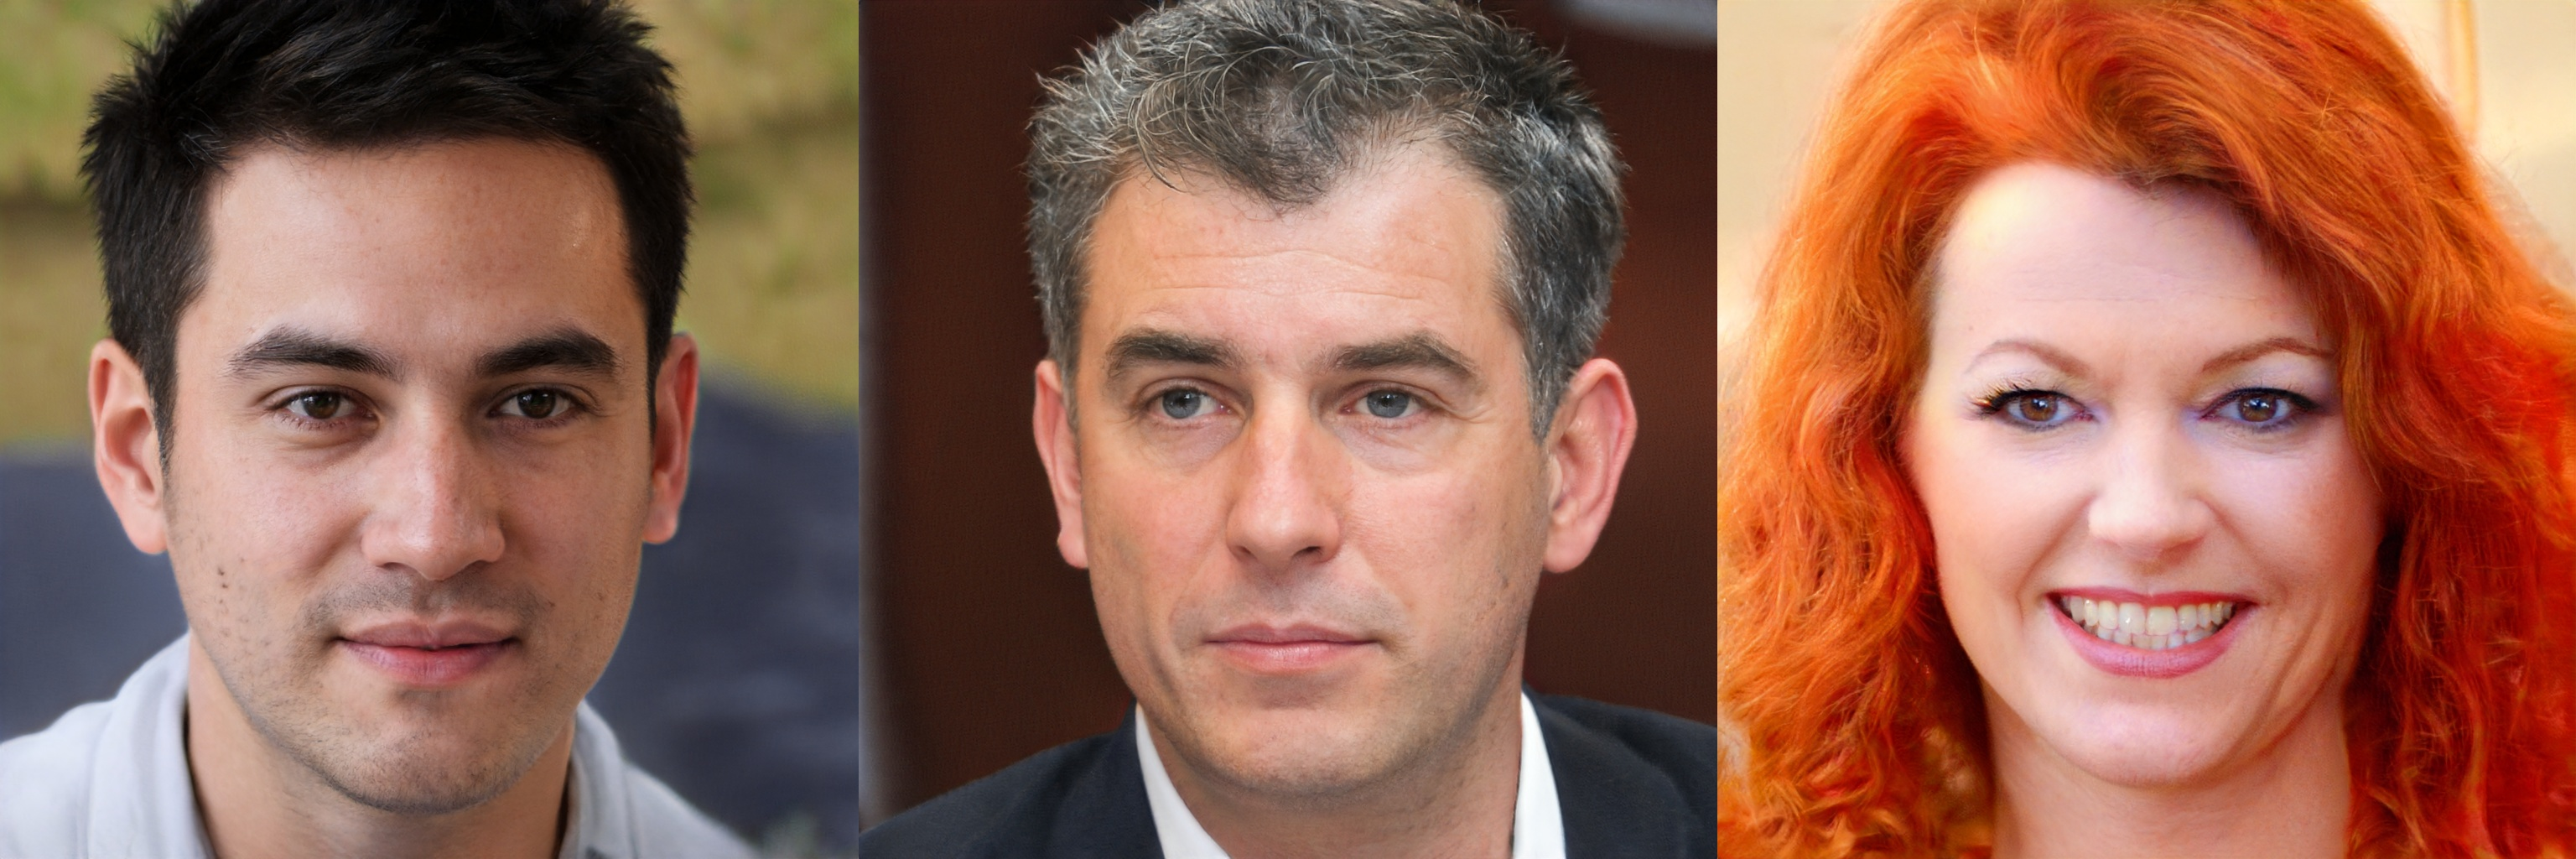
\includegraphics[width=0.8\textwidth]{images/pose_results/faces.jpg}
    \caption{Example of input faces from previous stage.}
    \label{fig:input_pose}
    \end{figure}
    
    \begin{figure}[H]
    \centering
    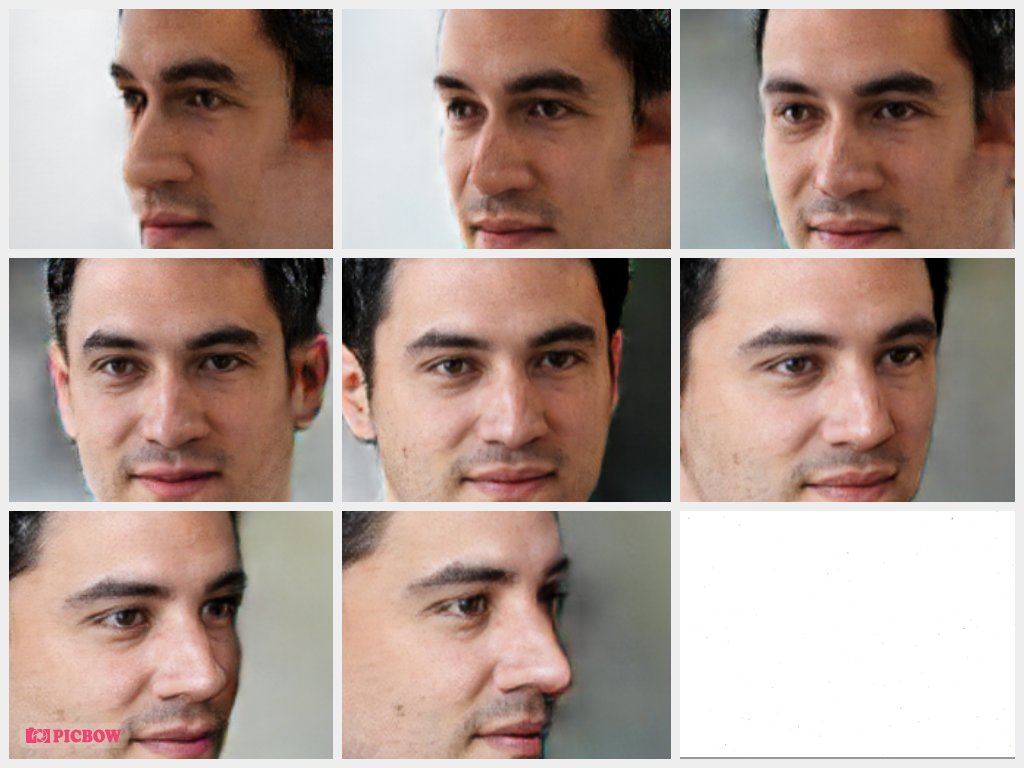
\includegraphics[width=0.8\textwidth]{images/pose_results/1.png}
    \caption{Example of output 8 poses for the first input face}
    \label{fig:pose_output1}
    \end{figure}
    
    \begin{figure}[H]
    \centering
    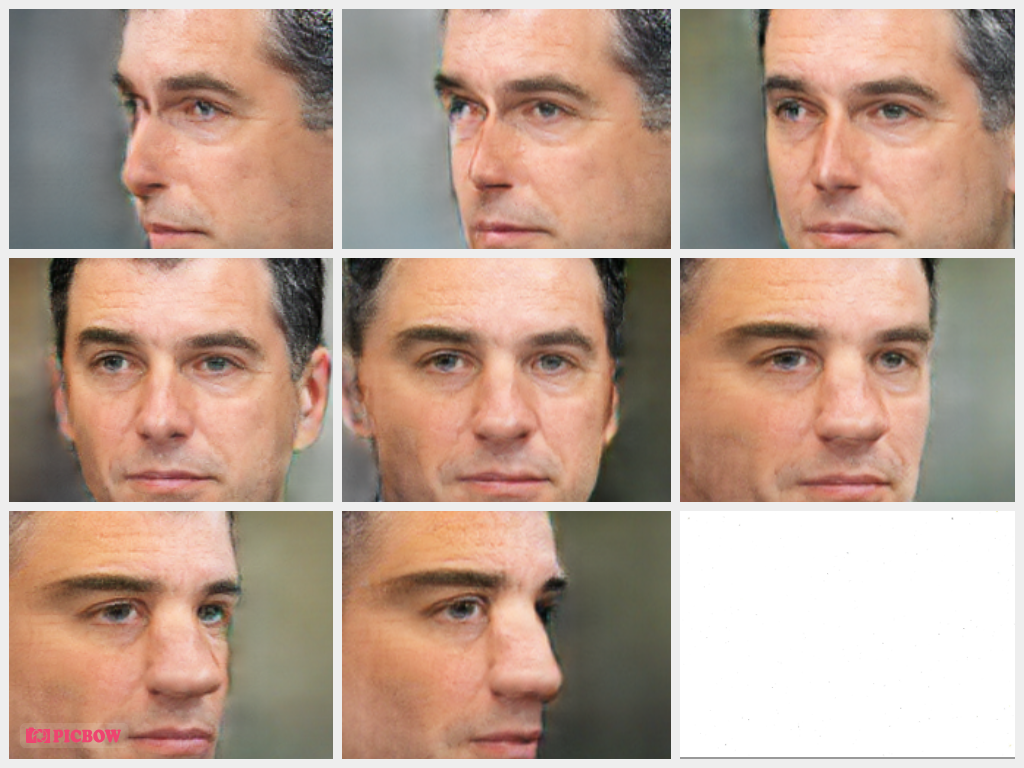
\includegraphics[width=0.8\textwidth]{images/pose_results/2.png}
    \caption{Example of output 8 poses for the second input face.}
    \label{fig:pose_output2}
    \end{figure}
    
    \begin{figure}[H]
    \centering
    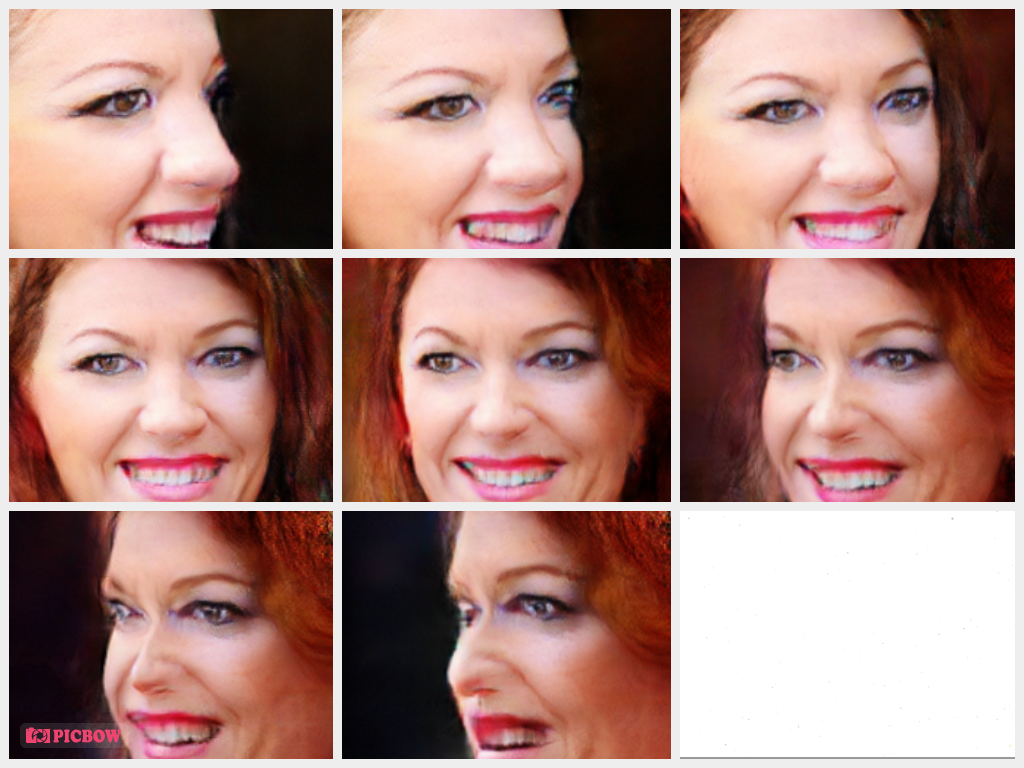
\includegraphics[width=0.8\textwidth]{images/pose_results/3.png}
    \caption{Example of output 8 poses for the third input face.}
    \label{fig:pose_output3}
    \end{figure}

\end{itemize}

\subsubsection{Integration Testing}
The integration of the whole system into a web application is tested qualitatively and quantitatively. In this section, we show the visual results of our system in an \emph{end-to-end} manner. However, we show the quantitative metrics in the comparison with previous work. 

Figures \ref{fig:correct_1} and \ref{fig:correct_2} show correct results of \textbf{face generation} in an \emph{end-to-end} manner using our final \emph{web application}, which contains our complete pipeline. We can see that the results samples are of high accuracy and fidelity. However, of course, the system is \emph{not} $100\%$ accurate. From our extensive testing to the system, we notice $4 types$ of failures, described visually in figure \ref{fig:incorrect}. These failures are listed as follows :
\begin{enumerate}
    \item Failures due to \textbf{contradicting facial features}. As in the \emph{top-left} image, as \emph{rosy cheeks} are very hard to capture with \emph{black skin color}.
    \item Failures due to \textbf{excessive navigation on directions}. As in the \emph{top-right} image, which is very unclear and of low quality with many visual artifacts.
    \item Failures due to \textbf{random initialization}. As in the \emph{bottom-left} image, where sometimes bad initial latent vector can cause the output to be visually inconsistent with many visual artifacts.
    \item Failures due to \textbf{sequential latent manipulation}. As in the \emph{bottom-right} image, where navigation on one direction (\emph{wavy hair}) cancel the navigation on another direction (\emph{short hair}).
\end{enumerate}

\begin{figure}[H]
    \centering
    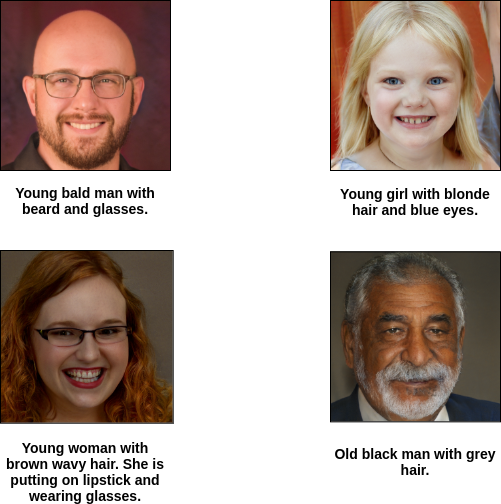
\includegraphics[width=0.8\textwidth]{images/correct-results_1.png}
    \caption{Samples of correctly generated face portrait from textual description.}
    \label{fig:correct_1}
\end{figure}

\begin{figure}[H]
    \centering
    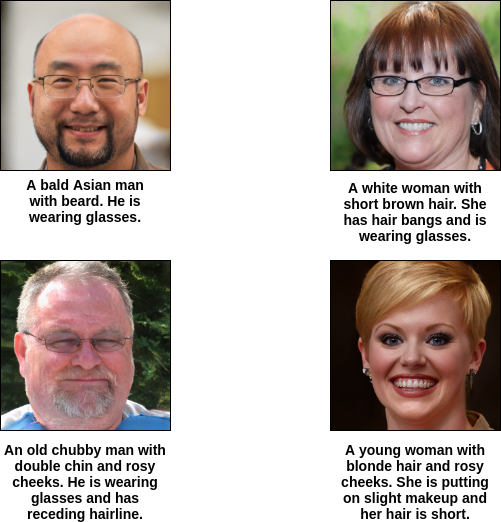
\includegraphics[width=0.8\textwidth]{images/correct-results_2.png}
    \caption{Samples of correctly generated face portrait from textual description.}
    \label{fig:correct_2}
\end{figure}

\begin{figure}[H]
    \centering
    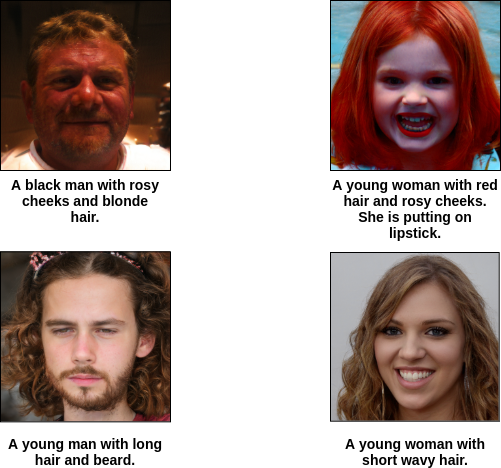
\includegraphics[width=0.8\textwidth]{images/incorrect-results.png}
    \caption{Samples of incorrectly generated face portrait from textual description.}
    \label{fig:incorrect}
\end{figure}

\subsection{Testing Schedule}
Our testing process is scheduled as follows :
\begin{itemize}
    \item First, we conducted the initial testing on the $3$ core modules, while being iteratively designed, until they converged to decent results.
    \item We, then, did the integration testing on these modules separately.
    \item After so, the rest of the system modules were designed and tested separately.
    \item Finally, the whole system was integrated into a single web application and complete testing of the whole system functionalities was conducted.
\end{itemize}

\subsection{Comparative Results to Previous Work}
First of all, it's worth mentioning that our system considers \emph{more facial features} than all previous research that worked on latent manipulation. As mentioned before, we compare our results quantitatively with $3$ baselines, using \textbf{FID score}, \textbf{average LPIPS} and \textbf{execution time}.

Table \ref{tab:fid} and plot \ref{fig:fid} show the comparison of our system to \texttt{StyleGAN2} and \texttt{Image2StyleGAN}. We couldn't include \texttt{Faces à la Carte} in this comparison, as the authors didn't include it in the paper. Also, we couldn't replicate their work, as they didn't provide any specific details about the implementation. We can see that as the number of test images increases, the overall quality of the images increases (\emph{FID} score decreases). Our system performs better than \texttt{Image2StyleGAN}, but worse than the original \texttt{StyleGAN2}, because it is just image generation from random vector with no \emph{latent manipulation} (fewer artifacts).

\begin{table}[ht]
\centering
\caption{FID scores comparison on different number of test images (lower is better).}
\begin{tabular}[t]{| c | c | c | c |}
\hline
Test Size & StyleGAN2 & Image2StyleGAN & Retratista \\
\hline \hline
50 & 129.15 & 179.58 & 151.58 \\
\hline
100 & 104.29 & 150.54 & 132.54 \\
\hline
200 & 95.25 & 136.45 & 114.45 \\
\hline
300 & 92.44 & 134.04 & 113.04 \\
\hline
400 & 86.37 & 121.59 & 100.59 \\
\hline
500 & 80.09 & 119.02 & 99.02 \\
\hline
\end{tabular}
\label{tab:fid}
\end{table}

\begin{figure}[H]
    \centering
    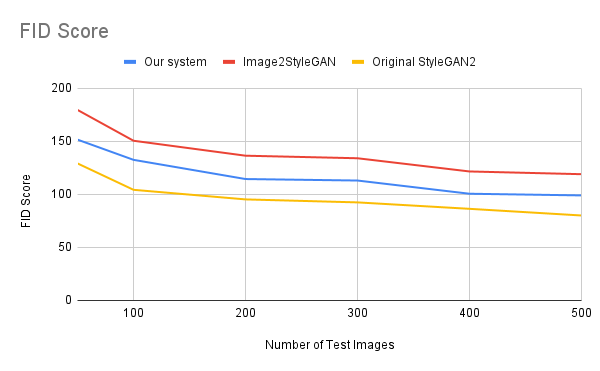
\includegraphics[width=0.8\textwidth]{images/fid_score.png}
    \caption{Plot of FID score of different pipelines against different number of test images (lower is better).}
    \label{fig:fid}
\end{figure}

Next, we compare our system with \texttt{Faces à la Carte} using the only metric, the authors provided, which \emph{LPIPS}. We can see from table \ref{tab:lpips_comp} that our system yields lower overall \emph{LPIPS}, which is better. However, we have higher error margin than \texttt{Faces à la Carte}.

\begin{table}[ht]
\centering
\caption{LPIPS comparison with Faces à la Carte (lower is better).}
\begin{tabular}[t]{| c | c |}
\hline
Retratista & Faces à la Carte \\
\hline
\hline
0.595±0.008 & 0.634±0.005 \\
\hline
\end{tabular}
\label{tab:lpips_comp}
\end{table}

Finally, table \ref{tab:exec_time} shows the execution time of different core stages of our system. We can see that the overall \emph{text-to-face generation} process takes only about $0.2$ seconds on an \emph{Nvidia GTX 1080 ti}. However, the web application can take from $1$ second up to multiple seconds to generate a face portrait (from any description) using the same GPU, depending on the \emph{connectivity} with the server. Meanwhile, our \emph{multiple head poses generation} module takes around $2$ seconds to generate a single pose on the same GPU as well. Most of the application backend runs on \emph{CUDA GPUs}. The whole system without \textbf{multiple head poses generation} module occupies around $5.5$ \emph{GB} of \emph{VRAM}. Meanwhile, this module occupies up to $3$ \emph{GB}. So, in total, the whole system occupies between $8$ to $9$ \emph{GB} of \emph{VRAM}.

\begin{table}[ht]
\centering
\caption{The execution time of different stages of the core of our system (measured in seconds).}
\begin{tabular}[t]{| c | c | c |}
\hline
Text Processing & Latent Manipulation & Face Generation \\
\hline
\hline
0.048 & 0.11 & 0.024 \\
\hline
\end{tabular}
\label{tab:exec_time}
\end{table}


\newpage

\section{Conclusions and Future Work}
Our system offers an innovative solution that leverages the power of \emph{Deep Learning}, \emph{Generative Adversarial Networks}, \emph{Computer Vision} and \emph{Natural Language Processing} to build an automated, fast and robust system for face generation and identification from various types of description. We push our pipeline to be as flexible and accurate as possible. Also we managed to overcome most of the challenges that faced us during building the system. Face generation and manipulation using voice, text and manual input are feasible in an automated way within few seconds. Moreover, our system considers a sufficient set of facial features to enable describing faces in an accurate way. Finally, our system is very flexible to add more facial features and further improve the results given enough resources and time.

\subsection{Faced Challenges}
Throughout the project, we faced many challenges. Basically, the challenges are related to \emph{data scarcity}, \emph{few related research work}, \emph{architectural complexity} and \emph{facial attributes}.

\subsubsection{Data Scarcity}
One of the main challenges of our project is data scarcity. No open-source source datasets exist for \emph{text-face} pairs, except only one dataset (\textbf{Face2Text}). We had to contact the authors, who kindly gave us an access for the dataset. Unfortunately, the dataset contains only $4000$ text-face pairs, which are not enough at all to conduct experiments or build the system. Consequently, we built our system in stages, as mentioned before. However, the \emph{text processing} module required a dataset, as it's completely supervised. Consequently, we built our face textual description from scratch, as discussed above \ref{sec:text}.

\subsubsection{Few Related Research Work}
Although the problem of image generation is popular in the research community, only one work actually targets human face generation from description. This work \cite{wang2020faces} does not even provide enough information about the method implementation. Consequently, we had to come up with our own working pipeline to build the face generation from description. We gained a lot of insights from other research works related to image (face) manipulation and awesome \texttt{StyleGAN2} follow-up papers.

\subsubsection{Architectural Complexity}
Most of the architectures related to high quality image generation are very complex and slow at inference. This results in the difficulty of editing or tuning them to other purposes. Also, we have to keep our inference time as minimal as possible. So, we had to spend a lot of time trying to adapt only the relevant modules of these enormous architectures into our system to maintain both time and memory complexity.

\subsubsection{Facial Attributes and Entanglement}
As mentioned before, the choice of facial attributes and the entanglement between them are the most difficult challenges of our project. We had to spend some time researching to select a set of facial attributes that correctly and sufficiently describes a human face. We came up with $32$ facial features for face generation and $38$ ($32$ + $6$ new) facial features for refinement. However, we were left with the entanglement challenge, because all open-source faces datasets contain real human faces. Real human faces contain natural entanglement between facial attributes. This results in features entanglement in the latent space of our generative model, which makes the process of feature directions extraction very difficult. We tried to solve this entanglement problem with various techniques and reached good results. However, the problem is not $100\%$ solved.

\subsection{Gained Experience}
Throughout our work on this project, we were exposed to numerous research works. We read lots of scientific research papers and articles, gained insights from many of them and adapted their techniques to our work. Also, we had the chance to work with multiple tools and technologies including, but not limited to, \emph{Python}, \emph{C/C++}, \emph{JavaScript}, \emph{PyTorch}, \emph{OpenCV}, \emph{REST APIs} and \emph{Docker}. Moreover, we gained a lot of experience from integrating such complex architectures into a single software.

\subsection{Conclusions}
Through the project, we managed to build a complete system that provides an automated, fast and robust way to generate and identify human faces from bare description. We consider voice, text and manual descriptions. Also, we formulated our system into a web application with a simple web user interface, where the user can input his preferred face description to be generated within few seconds. Then, the user is able to refine the generated face and render it in multiple poses for more identification. While being automated and accurate, our system suffers from some downsides as well. The facial features entanglement can still affect the output face portraits in some cases. Also, we tried to consider as much facial features as possible, however there can be even more features to include.

\subsection{Future Work}
Our work is flexible to changes and can be extended in various ways. To tackle the problem of entanglement, \texttt{StyleGAN2} synthesis network can be tuned using synthetic face images generated from \textbf{Epic's MetaHuman Creator}. This exposes the latent space to more generic faces with different facial features, which can help reducing entanglement and overlapping between feature clusters. Consequently, the set of facial features can be expanded to include more fine details about the human face. Following these methods, the system can be extended to generate fine-detailed human face portraits better than professional portraitists and within minimal time.


\newpage

%----------------------------------------------------------------------------------------
%	REFERENCES SECTION
%----------------------------------------------------------------------------------------

\medskip

\bibliographystyle{unsrt}
\bibliography{book}

\newpage

%----------------------------------------------------------------------------------------
%	APPENDIX SECTIONS
%----------------------------------------------------------------------------------------

\appendix

\section{Development Platforms and Tools}
Our project is completely software, so we discuss the software tools and packages used to develop our system.

\subsection{Software Tools}

\subsubsection{Ready-made Models}

\paragraph{Facial Landmark Detection Model}
The facial landmark detection model, used to extract some the feature directions, is completely ready-made. We used the open-source implementation of \textbf{High-resolution networks (HRNets) for facial landmark detection} \cite{sun2019highresolution} to do the landmark detection task, in order to get different facial distances and sizes.

\paragraph{Neural Face Renderer}
We used a ready-made neural network model for rendering $3D$ faces from $2D$ images to perform face rotation. This model is an open-source \emph{PyTorch} implementation for \textbf{Neural 3D Mesh Renderer} \cite{kato2017neural}.

\subsubsection{Frameworks and Packages}

\paragraph{PyTorch}
An highly-optimized open-source \emph{ML} library used to implement, train and deploy all \emph{DL} models used in our system.

\paragraph{OpenCV}
An open-source library for optimized image processing and computer vision applications. It's used in facial attributes classification in feature directions extraction.

\paragraph{Flask}
An open-source \emph{Python} framework, used to implement the server \emph{API} endpoints.

\paragraph{Vuejs}
An open-source \emph{JavaScript} framework, used to implement the web user interface.

\paragraph{Docker}
An open-source software used for containerization. It has been used throughout the project and through deployment for automation and to handle conflicting dependencies.


\section{Use Cases}

\begin{figure}[H]
    \centering
    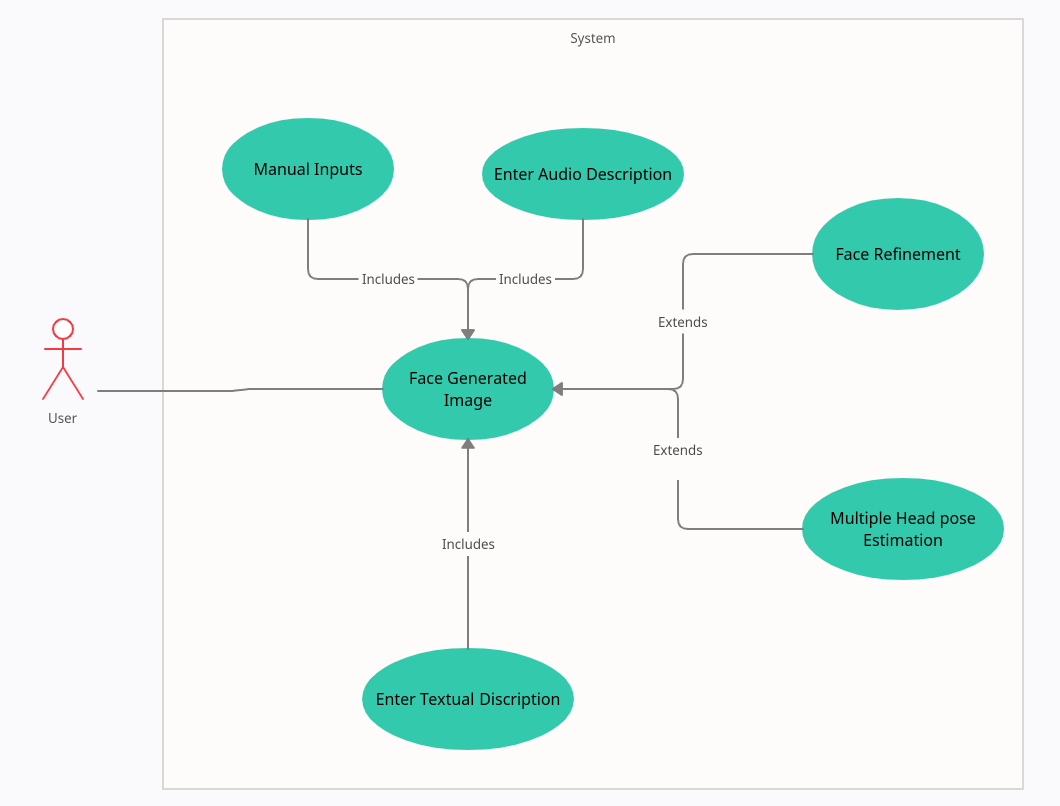
\includegraphics[width=\textwidth]{images/Puml.png}
    \caption{UML diagram for our application.}
    \label{fig:UMLD}
\end{figure}

As mentioned before, our application can be used in police station or any organization responsible for missing people like International Center for Missing and Exploited Children and many other organizations.
Also, Archaeological and Historical Researchers will be willing to use our app as it will help them to identify the facial description on the mummies using images not only textual descriptions.

\section{User Guide}
\subsection{Main Page}
In this page as shown in figure \ref{fig:user-main}, the user can 

\begin{enumerate}
    \item choose from a menu the generation mode that he or she wants.
    \item navigate to the demo and help page from the bar in the header.
\end{enumerate}
    
\begin{figure}[H]
    \centering
    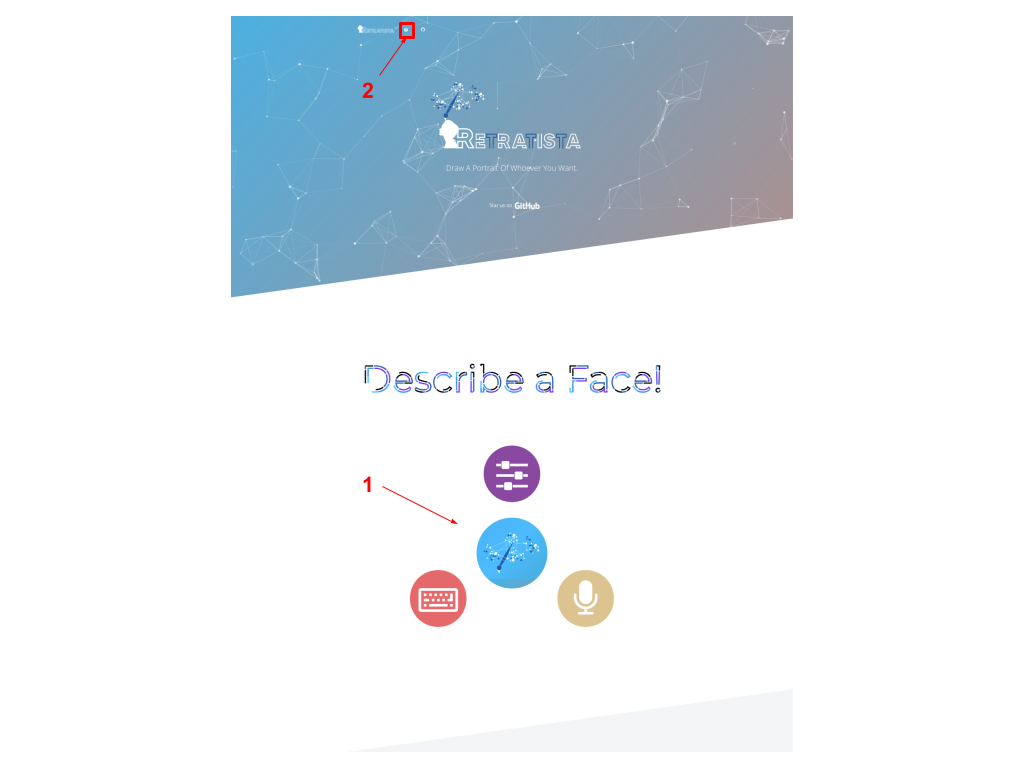
\includegraphics[width=1.0\textwidth]{images/guide/main.png}
    \caption{Main Page}
    \label{fig:user-main}
\end{figure}


\subsection{Voice Description Page}
In this page as shown in figure \ref{fig:user-voice}, the user can 

\begin{enumerate}
    \item describe a face using his voice.
    \item edit the description textually.
    \item generate the described face.
    \item route to refine page after generation.
    \item route to head poses page after generation.
\end{enumerate}

\begin{figure}[H]
    \centering
    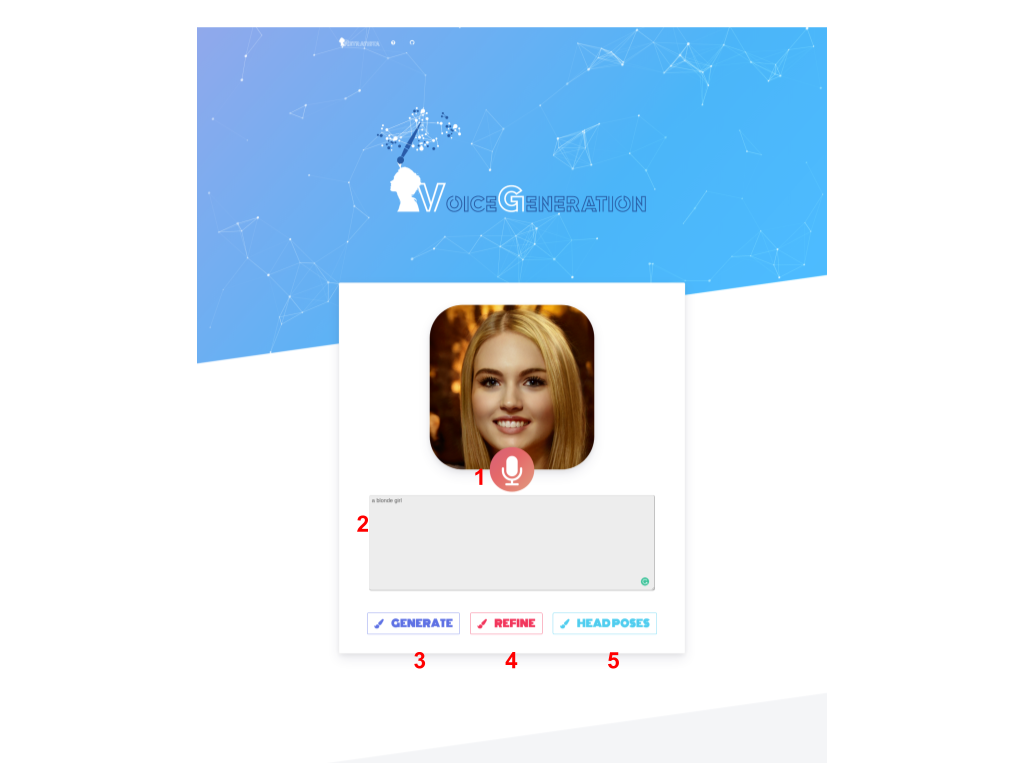
\includegraphics[width=1.0\textwidth]{images/guide/voice.png}
    \caption{Voice Description Page}
    \label{fig:user-voice}
\end{figure}


\subsection{Text Description Page}
In this page as shown in figure \ref{fig:user-text}, the user can 

\begin{enumerate}
    \item describe a face textually.
    \item generate the described face.
    \item route to refine page after generation.
    \item route to head poses page after generation.
\end{enumerate}

\begin{figure}[H]
    \centering
    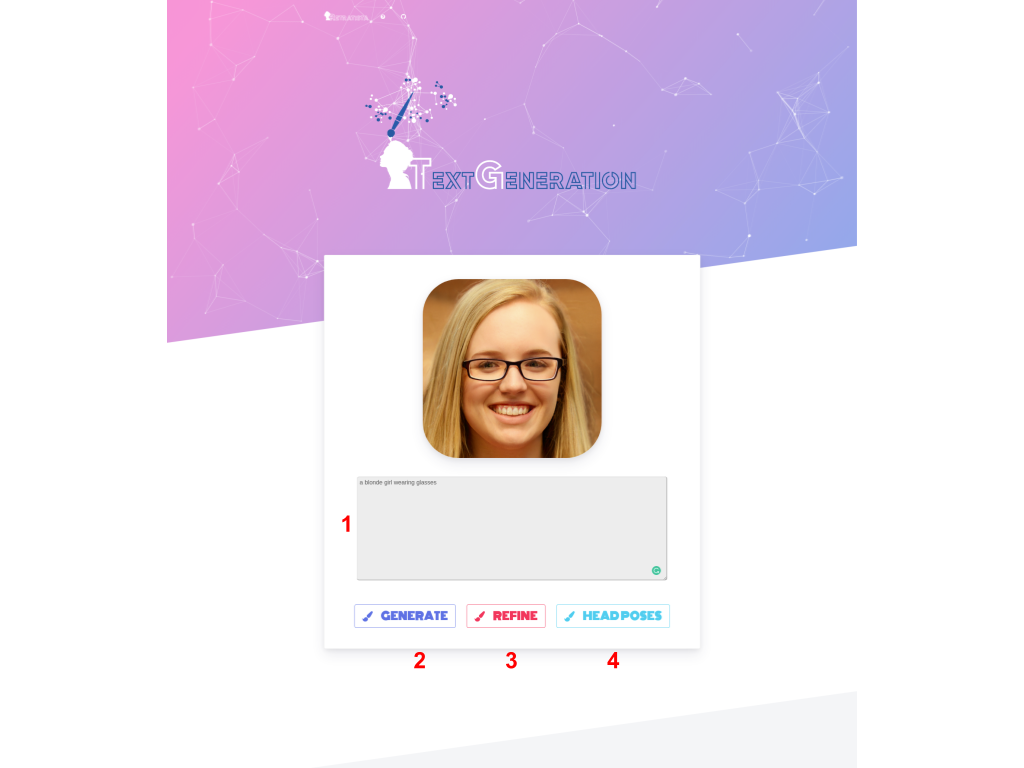
\includegraphics[width=1.0\textwidth]{images/guide/text.png}
    \caption{Text Description Page}
    \label{fig:user-text}
\end{figure}


\subsection{Refine Page}
In this page as shown in figure \ref{fig:user-refine} for refinement of age attribute, the user can 

\begin{enumerate}
    \item navigate in 39 different facial attributes to get the actual intended face.
    \item route to head poses page after refinement.
\end{enumerate}

\begin{figure}[H]
    \centering
    \includegraphics[width=0.7\textwidth]{images/website/refine.png}
    \caption{Refine Page}
    \label{fig:user-refine}
\end{figure}


\subsection{Head Pose Page}
In this page as shown in figure \ref{fig:user-poses}, the user gets 8 different head poses for the same person for extra identification. 

\begin{figure}[H]
    \centering
    \includegraphics[width=0.9\textwidth]{images/guide/poses.png}
    \caption{Head Pose Page}
    \label{fig:user-poses}
\end{figure}


\subsection{Demo Page}
This Page is a help aid for the user to know how to use the application and to support the user with some extra information about the project, such as
\begin{itemize}
    \item Why is Retratista important?
    \item Statistics
    \item Project Features
    \item How To Use?
    \item Result Samples
    \item Team
\end{itemize}


\section{Feasibility Study}
\subsection{Technical Feasibility}

To conduct this project knowledge base in the field of image processing and mathematics is required, to build on the knowledge in artificial intelligence, the use of generative adversarial networks and supervised learning to build and improve the models. Also, experience in web design and launching to represent our product to any user or organization, so that they buy it. We used our devices to train the models besides the online free service, such as \emph{Google Colab}. Additionally most of the developed models were guided by published research papers, therefore indicating and emphasizing the feasibility of the solution.

\subsection{Operational Feasibility}

As mentioned before, we deal with two types of users. One uses the application for special purposes; finding missing people or identifying the image of some ancient king or queen, so they need to have at least one PC with VRAM 11GB or more, to be able to run the application which will cost around \$1500 to \$2000 or more depends on the number of PCs will be used and their specifications. For the other type of users we can deploy the app for free as a trial, then a little expense is asked from subscribed users so that the deployment cost is covered with profits. 

\subsection{Legal Feasibility}

The development of the project depends on publicly available libraries and software tools, like \emph{PyTorch}, \emph{OpenCV}, \emph{Flask} and \emph{VueJS}. All the pretrained models used are open sources and legal to be used for any product. All datasets used to train any written model are public for any commercial use or made by us. The devices used to train those models are our own or on \emph{Google Colab}, which is also public for any use.

\subsection{ SWOT Analysis }

\subsubsection{Strength (S)}

\begin{itemize}
    \item Fast.
    \item Automated.
    \item Easy-to-use.
    \item Realistic results.
    \item Containing a sufficient set of features to describe a human face.
\end{itemize}

\subsubsection{Weaknesses (W)}

\begin{itemize}
    \item Facial features entanglement.
    \item High \emph{VRAM} usage.
    \item Sometimes results can be inaccurate.
\end{itemize}

\subsubsection{Opportunities (O)} 

\begin{itemize}
    \item No competitors.
    \item Fast and automated.
\end{itemize}

\subsubsection{Threats (T)}

\begin{itemize}
    \item Lack of datasets.
    \item High cost.
\end{itemize}


%**********************************************%

\end{document}